\documentclass[12pt,a4paper,twoside,titlepage]{report}
\usepackage{mi_estilo} % donde voy metiendo paquetes de estilo
\usepackage{titlesec} % formatear titulos
\titleformat{\chapter}[hang]{\normalfont\huge\bfseries}{\thechapter}{20pt}{\huge} % para quitar lo de Chapter al inicio de cada capitulo
\titlespacing*{\chapter}{0pt}{10pt}{15pt} % ajustar margenes titulos
\titlespacing*{\section}{0pt}{0pt}{0pt} % ajustar margenes títulos
\DeclareUnicodeCharacter{2212}{-} % resolver un error que me daba
\DeclareMathOperator{\Tr}{Tr} % crear operador Traza
\usepackage{xpatch} % para que hepnames funcione en LaTeX v2020
\makeatletter
\xpatchcmd\@HepConStyle
 {\edef\@upcode{\updefault}}
 {\ifdefined\shapedefault\edef\@upcode{\shapedefault}\else\edef\@upcode{\updefault}\fi}
 {}{}
\makeatother

\begin{document}
	\renewcommand{\listtablename}{Índice de tablas}
	\pagenumbering{roman}
	\begin{titlepage}

\newcommand{\HRule}{\rule{\linewidth}{0.5mm}} % Defines a new command for the horizontal lines, change thickness here

\center % Center everything on the page

%----------------------------------------------------------------------------------------
%	HEADING SECTIONS
%----------------------------------------------------------------------------------------

\textsc{\LARGE Trabajo fin de Grado}\\[1.8cm] % Name of your university/college

%----------------------------------------------------------------------------------------
%	LOGO SECTION
%----------------------------------------------------------------------------------------
\includesvg[width=0.6\textwidth]{{C:/Users/Carmen/Desktop/Universidad/TFG/Borradores/svg/logo_us}}\\[1.4cm]

%----------------------------------------------------------------------------------------

%----------------------------------------------------------------------------------------
%	TITLE SECTION
%----------------------------------------------------------------------------------------

\HRule \\[0.2cm]
{ \Large \bfseries
Mesones K: Extrañeza,\\[0cm]
Interacción Débil y Violación CP}\\[0.3cm]
\HRule \\[1.5cm]

%----------------------------------------------------------------------------------------
%	AUTHOR SECTION
%----------------------------------------------------------------------------------------

\begin{minipage}{0.4\textwidth}
\begin{flushleft} \large
%\vspace{9mm}
\emph{Autor:}\\
Carmen Sánchez Pérez
\end{flushleft}
\end{minipage}
~
\begin{minipage}{0.4\textwidth}
\begin{flushright} \large
\vspace{9mm}
\emph{Tutores:} \\
J. A. Caballero Carretero \\
G. D. Megías Vázquez
\end{flushright}
\end{minipage}\\[2cm]

% If you don't want a supervisor, uncomment the two lines below and remove the section above
%\Large \emph{Author:}\\
%John \textsc{Smith}\\[3cm] % Your name

%----------------------------------------------------------------------------------------
%	DATE SECTION
%----------------------------------------------------------------------------------------

{\large \today}\\[2cm] % Date, change the \today to a set date if you want to be precise



\vfill % Fill the rest of the page with whitespace

\end{titlepage}

\emptyPage


\begin{minipage}{0.3\textwidth}
\begin{flushleft}
\vspace{3cm}

\emph{En agradecimiento:}

\end{flushleft}
\end{minipage}
~
\begin{minipage}{0.6\textwidth}
\begin{flushright}
\vspace{15cm}

\scriptsize
\emph{A mis amigos, los que viven fuera y los de aquí, }\\
\emph{en especial a Noelia Martín Zorrero y a Ana Valadés Alcaraz,}\\
\emph{mis dos hermanas de distinta sangre, por apoyarme y enseñarme tanto,}\\
\emph{incluso en la distancia y tras tantos años.}\\[1cm]

\emph{A mi pareja y compañero de vida, Aythami Sosa Alemán,}\\
\emph{por todo su amor y por no dejar que tire nunca la toalla.}\\[1cm]

\emph{A mi familia, sobretodo a mis padres, Cati Pérez y Andrés Sánchez; }\\
\emph{y a mis hermanos, Belén y Pedro, por animarme y creer en mí siempre.}\\

\end{flushright}
\end{minipage}\\[2cm]
\vfill

\thispagestyle{empty}



	\tableofcontents
	\listoffigures
	\addcontentsline{toc}{chapter}{Índice de figuras y tablas}
	\begingroup
	\let\clearpage\relax % para unir lof y lot en una página
	\listoftables
	\endgroup
	\chapter*{Resumen}
\addcontentsline{toc}{chapter}{Resumen/Abstract}\label{cap:abstract}

Este documento se presenta como un estudio en detalle de lo que se conoce en Física de Partículas como mesones $\PK$ o kaones. La fama de los mesones $\PK$ radica en que fueron las primeras partículas en las cuales se detectó un comportamiento muy inusual: los mesones $\PK$ se forman gracias a la Interacción Fuerte, pero decaen por Interacción Débil. Por este motivo, se denominaron partículas extrañas y supuso la introducción de un nuevo número cuántico, la extrañeza $S$. Además, dado que decaen por interacción débil, pueden presentar violación de la simetría CP y, por tanto, oscilaciones de sabor. A pesar de que hoy en día también se han observado estos fenómenos en otras partículas, los mesones $\PK$ siguen actualmente jugando un papel muy importante y útil para estudiar las interacciones fundamentales. 
\vspace{2cm}

{\let\clearpage\relax\chapter*{Abstract}}
This document presents itself as thorough study of what is known in Particle Physics as $\PK$-mesons or Kaons. $\PK$-mesons renown lies in the fact that they were the first particles in which a very unusual behaviour was detected: $\PK$-mesons are formed thanks to the Strong Interaction but decay by means of the Weak Interaction. For this reason, they were named strange particles and it led to the introduction of a new quantum number, the Strangeness $S$. Moreover, since $\PK$-mesons decay by Weak Interaction, they can present CP-symmetry violation and therefore, flavor oscillations. In spite of this phenomena been observed  in other particles today, $\PK$-mesons still play an important and useful role in the study of Fundamentals Interactions nowadays.
	\chapter*{Objetivos y metodología}
\addcontentsline{toc}{chapter}{Objetivos y metodología}\label{cap:objetivos}

La propuesta de este Trabajo de Fin de Grado surge de la gran motivación que supuso en la asignatura de Física Nuclear y Partículas la realización de un proyecto en grupo conocido como ``Adopta una Partícula'' en el cuál se escogió el mesón K como partícula adoptada. Para nuestra sorpresa, esta partícula resultó ser de lo más fascinante.\\


Desde su descubrimiento, el mesón K ha constituido un rol fundamental en la Física de Partículas. No sólo fueron las primeras partículas extrañas que se detectaron, sino que ello supuso una revolución total para la Física moderna. Fueron los responsables de la introducción de la Extrañeza como nuevo número cuántico y ha servido de inspiración para sentar las bases del Modelo de Quarks, al requerir la existencia del quark extraño.

La teoría de Quarks, fomentada por el hallazgo de los mesones K, ha tenido numerosas consecuencias de suma importancia en el estudio de las Interacciones Fundamentales y, sobretodo, para la Interacción Débil. Gracias a ello ha sido posible predecir las posibles causas de violaciones de simetría, la existencia de nuevos quarks presentes en nuevas partículas y oscilaciones de sabor. \\


Por lo tanto, este trabajo pretende dar a conocer los mesones K en profundidad y detallar todas estas implicaciones que su descubrimiento ha traído consigo, con el objetivo de concentrar toda esa información en un único documento, facilitando el trabajo de los divulgadores e investigadores de este campo de la Física que necesiten o, simplemente, quieran conocer más acerca de estas partículas extrañas tan útiles y curiosas.\\


Para tal fin, tras unas breves pinceladas sobre el contexto histórico, comenzaremos con un estudio en tono cualitativo de la Extrañeza y la definición de mesón K en el Modelo de Quarks, seguido de un desarrollo más cuantitativo de la Interacción Débil, dónde haremos uso de su formalismo general. Finalmente, relacionaremos todo lo anterior con la violación de simetría CP y proporcionaremos algunos aspectos más actuales dónde se trabaja con mesones K.




	\clearpage % evitar error numeración romana en siguiente parte
	\pagenumbering{arabic}
	\renewcommand{\listtablename}{Índice de tablas}
\renewcommand{\tablename}{Tabla}

\chapter{Introducción}\label{cap:intro}
El período entre 1940-1950 fue clave para el desarrollo de la Física de Partículas debido a los numerosos descubrimientos que se llevaron a cabo. Yukawa había propuesto hace unos años atrás la existencia de una partícula portadora de la interacción fuerte, cuya masa estuviera entre la del protón y la del electrón y denominada por este motivo mesón (middle weight) \cite{Griffiths2008}.
 
En los años posteriores, los científicos no cesaron de realizar experimentos en las cámaras de niebla tratando de identificar la partícula de Yukawa \cite{Lattes}. Primero se descubrió en 1936 el muón $\Pmu$, una partícula cuya masa coincidía con la descrita por Yukawa pero que fue descartada al comprobar que su sección eficaz no era la propia de la Interacción Fuerte. En 1947, el grupo de investigación de Powell descubrió el mesón $\Ppi$ o pión, y esta vez la partícula sí coincidía con las predicciones de Yukawa. Sin embargo, este no fue el único descubrimiento realizado en 1947.

Los físicos británicos Rochester y Butler, se hallaban también ese año realizando experimentos en una cámara de niebla cuando observaron unos rastros inusuales en ella que tenían forma de $V$ invertida \cite{Nature1}. Este hecho supuso la primera observación de los mesones $\PK$. Decidieron repetir el experimento en los pirineos franceses, detectando decenas de estas nuevas partículas. En 1949, el grupo de Powell logró también observar un rastro parecido, indicando la presencia una partícula $V$, que luego decaía en tres piones \cite{Powell}. 

Con el paso del tiempo, las técnicas de detección de partículas mejoraron enormemente y durante la copiosa producción de estas partículas $V$ en los experimentos, se observó, entre otros curiosos fenómenos, que a pesar de que la interacción fuerte era la responsable de su formación, su larga vida indicaba que su desintegración se producía mediante interacción débil. Esta junto a otras características inusuales, hizo que estas partículas se ganaran el sobrenombre de extrañas. Desde entonces, se han detectado otras partículas extrañas tales como los bariones $\PSigma$ y $\Lambda^0$ \cite{Bardeen2012}.

Los científicos de la época propusieron varias teorías, pero finalmente se concluyó que era necesario introducir un nuevo número cuántico para darle explicación a este suceso: la extrañeza o strangeness $S$. 

Así pues, podemos concluir que los mesones $\PK$ son hadrones de tipo mesón; son partículas bosónicas que sienten la interacción fuerte y se caracterizan por tener espín entero (nulo en este caso) y número bariónico nulo (por ser mesones). Se consideran partículas ``estables'' porque, generalmente, decaen en hadrones más ligeros mediante interacción débil en lugar de por interacción fuerte o electromagnética y tienen vidas medias relativamente largas.

Actualmente se conocen 4 tipos de mesones $\PK$ distintos: las partículas $\PKp$ y $\PKz$ con sus respectivas antipartículas $\PKm$ y $\PaKz$. La siguiente tabla muestra un resumen de sus propiedades:\\

\begin{table}[h]
	\centering
	\begin{tabular}{l*{7}{c}r}
\hline
Partícula & $\PKp$ & $\PKm$ & $\PKz$ & $\PaKz$ \\ 
\hline
Carga $Q$ & $1$ & $-1$ & $0$ & $0$\\
Masa $\SI{}{\MeVcsq}$ & $493,677$ & $493,677$ & $497,611$ & $497,611$\\
Isospín $I$ & $1/2$ & $1/2$ & $1/2$ & $1/2$ \\
3ª componente del Isoespín $I_3$ & $1/2$ & $-1/2$ & $-1/2$ & $1/2$ \\
Momento angular y paridad $J^\pi$ & $0^-$ & $0^-$ & $0^-$ & $0^-$ \\
Nº Bariónico $B$ & $0$ & $0$ & $0$ & $0$\\
Extrañeza $S$ & $1$ & $-1$ & $1$ & $-1$\\
spin $s$ & $0$ & $0$ & $0$ & $0$\\ 
\hline
	\end{tabular}
\caption[Propiedades y números cuánticos relevantes de los Mesones $\PK$]{Propiedades y números cuánticos relevantes de los Mesones $\PK$.\protect\footnotemark}
\label{tab:propiedades}
\end{table}

\footnotetext{Propiedades extraídas de \cite{tanabashi}, \cite{notas2020}.}

En los siguientes capítulos se detallan, en mayor profundidad, la propiedad de la extrañeza así como los decaimientos de los distintos mesones $\PK$ por interacción débil y sus repercusiones en la violación de simetría CP.

	\chapter{Extrañeza}\label{cap:strangeness}

Como se comentó anteriormente, los físicos británicos George Rochester y Clifford Butler, se hallaban tomando fotografías en una cámara de niebla en 1947, tratando de detectar partículas generadas por los rayos cósmicos al impactar sobre las moléculas de la atmósfera, cuando detectaron dos rastros en forma de $V$ invertida nunca observados hasta entonces, que sólo podían ser explicados por el decaimiento de una partícula neutra con masa entre 700 y 1600 veces mayor a la del electrón. 

En aquella época, ante la ausencia de aceleradores de partículas potentes, la búsqueda de partículas se realizaba estudiando los rayos cósmicos. Estos rayos no son más que radiación de alta energía procedente del espacio exterior. Cuando estos inciden en las distintas capas de la atmósfera producen una serie de reacciones en cadena que da lugar a una cascada de partículas. Además, a mayor altitud, mayor es el flujo de rayos cósmicos que nos llegan, lo que facilita que un mayor número de partículas llegue al detector. Por este motivo, Rochester y Butler decidieron realizar nuevamente el experimento en los Pirineos Franceses, concretamente en el Observatorio \textit{Pic Du Midi}, y esta vez consiguieron detectar decenas de estas nuevas partículas. En un principio se las denominó partículas $V$ pero posteriormente pasaron a identificarse como mesones $K$ o kaones. \cite{Griffiths2008}

Para entender cómo lograron detectar los mesones $K$ por primera vez, hay que entender el funcionamiento de las cámaras de niebla. En estos dispositivos son entornos cerrados donde se llevaba a cabo el estudio de los rayos cósmicos: las partículas que componen los rayos atraviesan un volumen con vapor de agua sobresaturado contenido en dicho recinto cerrado. Las partículas con carga eléctrica producen una cierta ionización de aire provocando la condensación del vapor de agua a lo largo de la trayectoria.  Al situar la cámara de niebla en campos eléctricos y magnéticos, y estudiando las curvaturas de las trayectorias es posible obtener la carga eléctrica, la energía y la masa de las partículas.  Asimismo, como muchas partículas decaen en otras por ser inestables, estudiando la longitud de las trazas que dejan las partículas al decaer en la cámara de niebla, se puede deducir su vida media. \cite{notas2020}\\

En diciembre de 1947, se publicaron en la revista \textit{Nature} dos de las numerosas fotografías que habían tomado Rochester y Butler, las cuales podemos observar a continuación:



\begin{figure}[h]
	\centering
	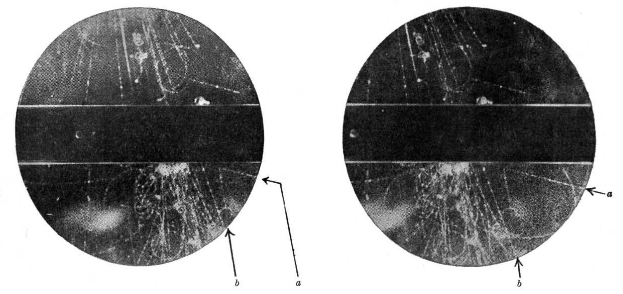
\includegraphics[width=0.8\textwidth]{C:/Users/Carmen/Desktop/Universidad/TFG/Borradores/img/rochester1.PNG}
	\caption[Fotografía 1 de la primera detección de los mesones $K$]
	{Primera fotografía estereoscópica publicada en la revista \textit{Nature}. \cite{Nature1}}
	\label{fig:nature1}
\end{figure}

\begin{figure}[h]
	\centering
	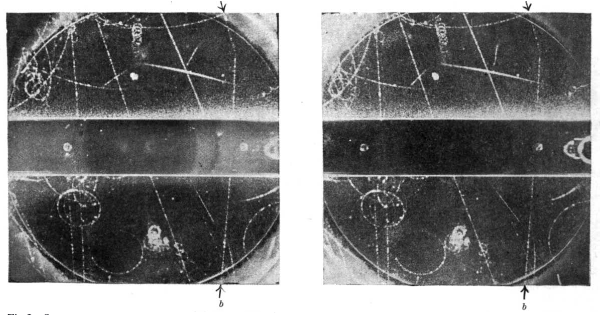
\includegraphics[width=0.8\textwidth]{C:/Users/Carmen/Desktop/Universidad/TFG/Borradores/img/rochester2.PNG}
	\caption[Fotografía 2 de la primera detección de los mesones $K$]
	{Segunda fotografía estereoscópica publicada en la revista \textit{Nature}. \cite{Nature1}}
	\label{fig:nature2}
\end{figure}


En la figura \ref{fig:nature1}, se observa como las partículas de rayos cósmicos entran por la parte superior izquierda y colisionan contra la placa de plomo, produciendo una partícula neutra, cuya presencia se hace evidente al decaer en otras partículas cargadas más ligeras, formando una ``V'' invertida en la parte inferior derecha, señalada mediante las marcas a y b. La figura \ref{fig:nature2} muestra un proceso similar pero esa vez, se produce una nueva partícula cargada (por entonces partícula-$\tau$) que decae en otras dos partículas más ligeras, una cargada y la otra neutra, apreciándose una desviación o ``kink'' en las trayectorias.\\

%Para entender las fotografías en mayor detalle, a continuación se muestra un esquema de uno de los procesos.

%\begin{figure}[h]
%	\centering
%	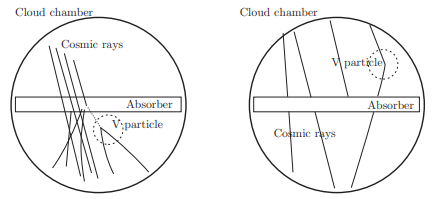
\includegraphics[width=0.8\textwidth]{C:/Users/Carmen/Desktop/Universidad/TFG/Borradores/img/esquema.PNG}
%	\caption[Esquema para entender las fotos estereoscópicas]
%	{Esquema del proceso observado en la primera fotografía estereoscópica. \cite{Griffiths2008}}
%	\label{fig:esquema1}
%\end{figure}

Años más tarde se comprobó que la primera fotografía \ref{fig:nature1} correspondía al proceso  $K^0 \rightarrow \pi^+$ +  $\pi^- $ y la segunda fotografía (\ref{fig:nature2}) a la reacción $K^+ \rightarrow \mu^+$ + $\nu $.

El comienzo de los años 50 trajo consigo técnicas innovadoras de detección de partículas, como la cámara de burbujas, detectores de emulsión nuclear muy precisos y nuevos aceleradores más potentes. Estos nuevos dispositivos demostraron un gran avance tecnológico al permitir la producción casi en masa de las partículas descubiertas en la década anterior. 

De hecho, los mesones $K$ habían quedado un poco en el olvido durante los dos años posteriores a su descubrimiento hasta que en 1950 otros célebres físicos de partículas como Powell, empezaron a publicar trabajos donde también se apreciaban los trazos en forma de $V$ y las desviaciones, que evidenciaban la presencia de las partículas $V$ y $\tau$, respectivamente. Coincidían con Rochester y Butler en que estos eventos representaban el decaimiento espontáneo de partículas neutras y cargadas, desconocidas hasta entonces. 

\begin{figure}[h]
	\centering
	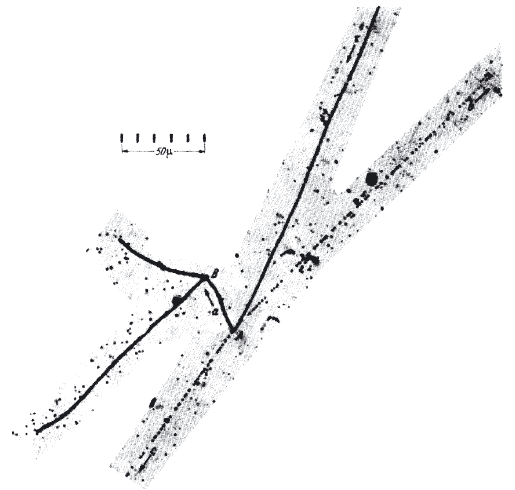
\includegraphics[width=0.5\textwidth]{C:/Users/Carmen/Desktop/Universidad/TFG/Borradores/img/powell.PNG}
	\caption[Fotografía de Powell mostrando una trayectoria ``kink'']
	{Fotografía publicada por el grupo de Powell en la revista \textit{Nature}. \cite{Griffiths2008}}
	\label{fig:powell}
\end{figure}

El proceso descubierto por Powell en \ref{fig:powell} mostraba como $K^+$ entrando desde arriba decae en el punto A en tres piones cargados, dos positivos y uno negativo. El $\pi^-$ provoca seguidamente una desintegración en B. El proceso descrito era: $K^+ \rightarrow \pi^+$ + $\pi^+$ +  $\pi^- $.

Sin embargo, la partícula $K^0$ primero fue conocida como $V^0$ y luego como $\theta^0$ antes de renombrarse finalmente como $K^0$, mientras que la partícula $K^+$ se denominó en un principio como $\tau^+$. Esto es debido a que los procesos de \ref{fig:nature1} y \ref{fig:powell} tenían estados finales con distinta paridad y por eso se pensaba que debía tratarse de partículas diferentes.

$\theta^0$ y $\tau^+$ no se identificaron como distintas versiones de una misma partícula hasta 1956, cuando se resolvió el conocido enigma $\tau$-$\theta$ al descubrir la violación de la paridad en la interacción débil, de la cual hablaremos más adelante. \cite{Griffiths2008}

En los años siguientes empezaron a clasificar las partículas $V$ y $\tau$ en función de la masa. Así, se determinó que los mesones $K$ correspondían a aquellas partículas con masa intermedia entre el pión y el protón, mientras que aquellas con masas intermedias entre el neutrón y el deuterón pasarían a conocerse como hiperones. 

Volviendo al inicio de los años 50, fue también entonces cuando empezaron hacerse notar los fenómenos inusuales que presentaban estas partículas y que fueron los responsables de que se las bautizara como partículas extrañas, pues nunca se habían manifestado en otras partículas. Las partículas extrañas incluyen no sólo los mesones $K$, sino también los hiperones $\Lambda$, $\Sigma$ y cascada $\Xi$, entre otros. Pero para lo que nos concierne en este documento, vamos a centrar nuestro estudio en los kaones.

La primera característica extraña, mencionada ya antes varias veces, es el hecho de que estas partículas, a pesar de producirse por interacción fuerte de forma muy numerosa, tenían vidas medias relativamente largas, por lo que se sospechaba que decaían mediante interacción débil. El otro suceso curioso es el de producción asociada, que consiste en que las partículas extrañas sólo se producen por pares.  

Tras muchos intentos fallidos de dar explicación a estos hechos, el físico holandés-estadounidense Abraham Pais sugirió, en 1952, que las partículas elementales debían tener una nueva propiedad o regla de selección, a la que denominó ``Regla par-impar''. Esta regla de selección debía de cumplirse siempre para la Interacción Fuerte y la Electromagnética, pero podía violarse en la Interacción Débil. A grandes rasgos, la regla consistía en asignar el número 0 a las partículas ``antiguas'' ($\pi$, nucleones, $\gamma$, leptones) y el número 1 a las partículas ``nuevas'' $K$ y $\Lambda$ (el resto de las partículas todavía se desconocían). Dado cualquier proceso, se suman los números asignados de las partículas en el estado inicial y luego las del estado final. En la interacción fuerte y electromagnética, el número total inicial y final deben ser ambos pares o ambos impares, mientras que, en la interacción débil, uno debe ser par y el otro impar. Esta propiedad también daba respuesta a por qué las partículas extrañas debían producirse en pares. \cite{Pais}

La evidencia experimental de la idea de Pais vino de la mano de Murray Gell-Mann y Kazuhiko Nishijima en 1953. Por un lado, indicaban que la ``Regla par-impar'' debía ser una consecuencia directa de la independencia de carga de las partículas $V$, que indicaba que la carga de estas partículas podía encontrarse en tres estados: neutro, positivo y negativo. Por otro lado, Gell-Mann propuso asignar un número entero de Isospín $I$ a los hiperones y un semientero a los mesones $K$. Nakano y Nishijima también hicieron esta misma propuesta casi paralelamente. Dependiendo de si el isospín $I$ y su tercera componente $I_3$ se conservan o no, podrá llevarse acabo la producción de partículas mediante Interacción Fuerte. \cite{nakano}

En 1955, Nishijima planteó, a partir de sus observaciones experimentales, que los mesones $K$ se podían organizar en dobletes de carga y, por tanto, podían obtenerse partículas $K$ con carga conjugada. $K^+$ y $K^0$ formaban un doblete de carga con $I=1/2$ e $I_3=1/2$ y $-1/2$ respectivamente y, además, ambas partículas podían definirse como funciones de onda complejas. Ello permitía establecer el doblete conjugado de sus antipartículas $K^-$ y $\overline{K^0}$, con $I_3=-1/2$ y $1/2$ respectivamente, relacionados entre sí mediante el operador conjugación de carga. Gell-Mann también llegó a conclusiones similares en 1956. Profundizaremos en mayor medida sobre este tema en los próximos capítulos. \cite{Nishijima1955}

Por otro lado, se comprobó que en todas las interacciones antes descritas se conservaba el número bariónico $B$.\protect\footnotemark    Asimismo, desarrollando toda esta teoría de la invariancia de carga para las partículas $V$ y para incluir la propiedad sugerida por Pais, se introdujo un nuevo número cuántico al que Gell-Mann denominó \textit{extrañeza} o \textit{Strangeness} $S$ (Nishijima lo denotaba como carga-$\eta$). Asignaron $S=1$ al doblete de partículas de mesones $K$ y $S=-1$ para el doblete de sus antipartículas. Este nuevo número cuántico resultaba últil para relacionar la carga con $I_3$ en partículas elementales, llegándose a una expresión conocida como la \textit{Fórmula de Gell-Mann-Nishijima}:

\footnotetext{Las teorías de Unificación afirman que el protón $p$ tiene vida finita aunque muy larga. Si decae, lo haría en un $e^+$ y en un $\pi^0$, violándose la conservación de $B$.}

\begin{equation}
Q=I_3+ \frac{B+S}{2}=I_3+\frac{Y}{2}
\end{equation}

Siendo $Y$ la \textit{hipercarga}, definida como $Y=B+S$ en un principio.

El teorema de Conservación de la Extrañeza se formuló a partir de las evidencias experimentales: $S$ debía conservarse en las Interacciones Fuerte y Electromagnética, pero podía ser violada en procesos ocurridos por Interacción Débil, tal y como había sugerido Pais con su \textit{Regla par-impar}.


\section{Extrañeza en el Modelo de Quarks}\label{cap:strangeness_quark_model}
\vspace{5mm}
Como hemos visto, el concepto de extrañeza se introdujo por motivos puramente fenomenológicos, gracias a las observaciones experimentales. Sin embargo, a través del Modelo de Quarks, la extrañeza obtiene su base teórica.

A principios de la década de los 60, y tras el descubrimiento de muchas partículas ``elementales'' se hizo necesario poner cierto orden haciendo uso de las simetrías. Las simetrías son útiles porque permiten clasificar de forma ordenada las partículas en función de sus propiedades. La rama de las matemáticas encargada de tratar con simetrías es la teoría de grupos. El isospín viene descrito por el grupo $SU(2)$, pero el descubrimiento de las partículas extrañas hizo necesario extender el concepto de isospín a una simetría superior.

Así pues, Gell-Mann y Ne'eman observaron que los valores de isospín y la hipercarga de los hadrones estaban relacionados entre sí, tal que los hadrones (mesones y bariones) aparecían en grupos, con el mismo espín y paridad y masas similares, denominados singletes (una partícula), octetes (ocho partículas) y decupletes (diez partículas).  Esta clasificación recibió el nombre de \textit{The Eightfold Way} o \textit{El Camino Óctuple}, concordaba con la estructura del grupo de simetría interna $SU(3)$ si fundamentaban las transformaciones en la independencia de carga de la interacción fuerte (isospín) y en la conservación de la extrañeza.\cite{notas2020} Las diversas representaciones del $SU(3)$, no sólo permitían la clasificación de las partículas en función de sus números cuánticos, sino que además, predecían la existencia de nuevas partículas aún por descubrir. 

Pero entonces, ¿por qué los hadrones se organizaban en estructuras con formas tan curiosas? La respuesta a esta pregunta se obtuvo en 1964, cuando Gell-Mann y Zweig, plantearon la posibilidad de que estas partículas, que en un principio se creían elementales, podrían presentar una estructura interna más compleja, pues habían observado ciertas propiedades en ellas que así lo sugerían. Gell-Mann bautizó a estos entes más fundamentales que constituían las partículas como \textit{quarks}.\cite{Griffiths2008} El quark presentaba tres estados internos o ``sabores'', llamados $u$ (\textit{up}), $d$ (\textit{down}) y $s$ (\textit{strange}), cada uno con un determinado valor de carga y extrañeza. Además, indicó que para cada quark $q$, existía su correspondiente antiquark $\overline{q}$ con números cuánticos aditivos opuestos. En la siguiente tabla se puede observar un resumen de sus propiedades:

\begin{table}[h]
	\centering
	\begin{tabular}{l*{8}{c}r}
\hline
Quark $(q)$ & Espín $s$ & Carga $Q$ & $I$ & $I_3$ & $S$ & $B$ & $Y$\\ 
\hline
Up $(u)$ & $1/2$ & $+2/3$ & $1/2$ & $+1/2$ & $0$ & $1/3$ & $1/3$\\
Down $(d)$ & $1/2$ & $-1/3$ & $1/2$ & $-1/2$ & $0$ & $1/3$ & $1/3$\\
Strange $(s)$ & $1/2$ & $-1/3$ & $0$ & $0$ & $-1$ & $1/3$ & $-2/3$\\
\hline
	\end{tabular}
\caption{Números cuánticos de los quarks. \cite{notas2020}} %\protect\footnotemark}
\label{tab:propiedades_quarks}
\end{table}

%\footnotetext{Recordemos que los respectivos antiquarks tienen números cuánticos opuestos.}

Así nació el \textit{Modelo de Quarks}, el cuál establecía que los bariones (antibariones) se componían de un conjunto de tres quarks (antiquarks) mientras que los mesones estaban formados por un quark y un antiquark. El \textit{The Eightfold Way} sólo era una consecuencia de las simetrías de sabor de los quarks, matemáticamente expresada mediante la simetría del grupo $SU(3)$. Las diferentes combinaciones de sabor daban lugar a las distintas partículas y sus propiedades.

En concreto, los mesones $K$ se representaban junto a los piones en un hexágono con que los clasifica según sus números cuánticos de carga $Q$ y extrañeza $S$, formando un octete pseudo-escalar.\footnote{Pseudo-escalar indica que los mesones tienen momento angular 0 y paridad negativa ($J^\pi = 0^-$).} Dicho octete está formado por el triplete de los piones y los dos dupletes de las partículas $K$ y sus antipartículas, aunando así todos los mesones ligeros en un mismo grupo. Para formar el octete de mesones, en cada vértice del hexágono se sitúa una partícula y en el centro del mismo se sitúan el pión neutro y el mesón $\eta$. En la siguiente figura se puede ver la representación de este octete:

\begin{figure}[h]
	\centering
	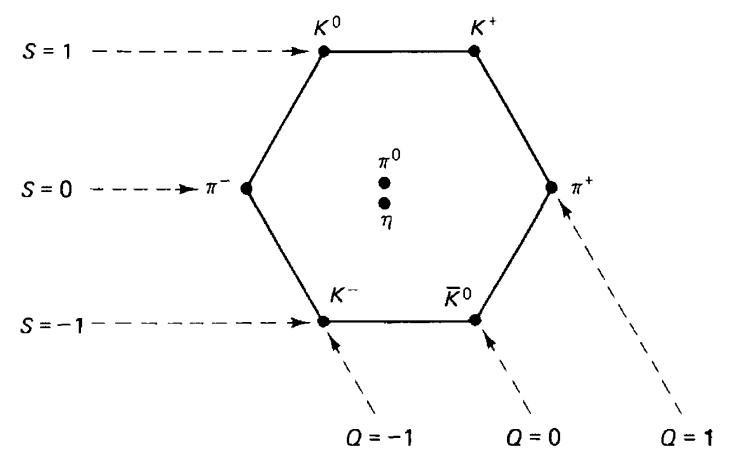
\includegraphics[width=0.65\textwidth]{C:/Users/Carmen/Desktop/Universidad/TFG/Borradores/img/octete.PNG}
	\caption[Octete de mesones]
	{Octete de mesones. \cite{Griffiths2008}}
	\label{fig:octete}
\end{figure}

Este octete muchas veces aparece representado como un nonete para incluir las nueve posibles combinaciones de $q$ y $\overline{q}$, al incluir el singlete de la partícula $\eta'$.

Por lo tanto, todas aquellas partículas en cuya composición estuviera presente el quark $s$, como en los kaones, presentaban un valor de extrañeza no nulo y podían considerarse partículas extrañas. La composición de quarks de los mesones $K$ es la siguiente:

\begin{table}[h]
	\centering
	\begin{tabular}{l*{2}{c}r}
\hline
Mesón & Quarks\\ 
\hline
$K^+$ & $u\overline{s}$\\
$K^-$ & $s\overline{u}$\\
$K^0$ & $d\overline{s}$\\
$\overline{K^0}$ & $s\overline{d}$\\
\hline
	\end{tabular}
\caption{Composición de quarks de los mesones $K$. \cite{notas2020}} 
\label{tab:mesonesK_quarks}
\end{table}

Conociendo esta composición y los números cuánticos de los quarks de la tabla \ref{tab:propiedades_quarks}, se obtienen fácilmente las propiedades de los mesones $K$ mostradas en la tabla \ref{tab:propiedades}.

Lo más destacable de los quarks es que son partículas fermiónicas, es decir tienen espín $1/2$. Sin embargo, la existencia de los bariones requiere la agrupación de tres quarks y esto, en un principio, parece contradecir el \textit{Principio de Exclusión de Pauli}. Para resolver esta paradoja, Greenberg introdujo el concepto de color: además de los tres sabores de quarks, estos también presentan tres colores $r$ (\textit{red}), $b$ (\textit{blue}) y $g$ (\textit{green}). Planteó que los bariones simplemente se forman con quarks de distinto color. Por lo tanto, ya no serían exactamente iguales y no se violaría el Principio de Pauli.\cite{Griffiths2008}  Además, a pesar de que los quarks son los constituyentes más fundamentales de la materia, no se han encontrado evidencias de la existencia de quarks aislados, es lo que conoce como confinamiento.\cite{Pais}

Con los años se han descubierto otros sabores de quarks, los llamados quarks pesados $c$ (\textit{charm}), $t$ (\textit{top}) y $b$ (\textit{botttom}). Esto ha requerido utilizar simetrías de orden superior al $SU(3)$ y modificar la definición de la hipercarga $Y$ para incluir estos nuevos sabores y poder clasificar las nuevas partículas descubiertas adecuadamente.

Gracias al Modelo de Quarks es posible describir la interacción entre partículas como interacciones entre los quarks que las componen. Los mesones $K$ se originan por la Interacción Fuerte. En esta interacción se producen intercambios de quarks entre los hadrones o se crean/aniquilan parejas quark-antiquark. La responsable de la interacción fuerte entre los quarks es su carga de color y la partícula portadora es el gluón.  Los quarks modifican su color al absorber o emitir un gluón pero no modifican su sabor (simetría de isospín). Las combinaciones antisimétricas de quarks frente al intercambio de color se atraen y las simétricas se repelen. Los gluones a su vez también tienen carga de color y pueden interactuar entre sí, lo que resulta en un aumento de la interacción fuerte con la distancia entre quarks y su confinamiento.\cite{notas2020} Por otro lado, los mesones $K$ decaen mediante la Interacción Débil. Estos procesos se pueden describir utilizando diagramas de Feynmann donde se aprecia el cambio de sabor de los quarks, que puede resultar o no en un cambio de extrañeza, dependiendo de qué quarks se crean y se aniquilan. Como este fenómeno es de suma importancia para los mesones $K$, dedicaremos el siguiente capítulo a tratar el tema de la Interacción Débil y la desintegración de estas partículas en detalle.\\



\section{Extrañeza en partículas <<no extrañas>>}
\label{cap:non-strange_particles}
\vspace{5mm}

Para finalizar este capítulo sobre la extrañeza, hay que mencionar que, si bien, en un primer momento, la composición más elemental de ciertos hadrones parece estar constituida únicamente por hasta tres sabores de quarks diferentes, estudios recientes han descubierto ciertas partículas que parecen presentar una estructura interna más compleja, que contienen toda una amplia variedad de sabores de quarks, antiquarks y gluones, pero de forma ``escondida''. Así lo manifiesta Ross D. Young en su artículo de la revista \textit{Nature} \cite{protonYoung}, donde se centra en explicar la extrañeza del protón, una partícula considerada originalmente como no extraña. 

La composición de quarks del protón es $uud$, sin embargo, los otros cuatro sabores también pueden estar ocultos en su estructura y afectar a sus propiedades, sobre todo a la distribución de carga y a la magnetización. El sabor oculto dominante en el protón se espera que sea $s$, pues tras $u$ y $d$, es el quark más ligero. De la \textit{cromodinámica cuántica} o \textit{QCD} (teoria que describe las interacciones entre quarks y gluones), se sabe que la cantidad neta de extrañeza debe ser siempre 0, así cada vez que se crea un quark, también se crea un antiquark $\overline{s}$, sólo que $\overline{s}$ aparece un poco más lejos del centro del protón con respecto a $s$, y esta asimetría afecta a su distribución de carga total. Además, la presencia de los quarks extraños en el protón hace que se incremente levemente su momento magnético, debido a la circulación neta de carga eléctrica negativa alrededor del eje de polarización del protón.\cite{protonYoung} Así lo han demostrado las simulaciones experimentales llevadas a cabo en el campo de la QCD.\\

\begin{figure}[h]
	\centering
	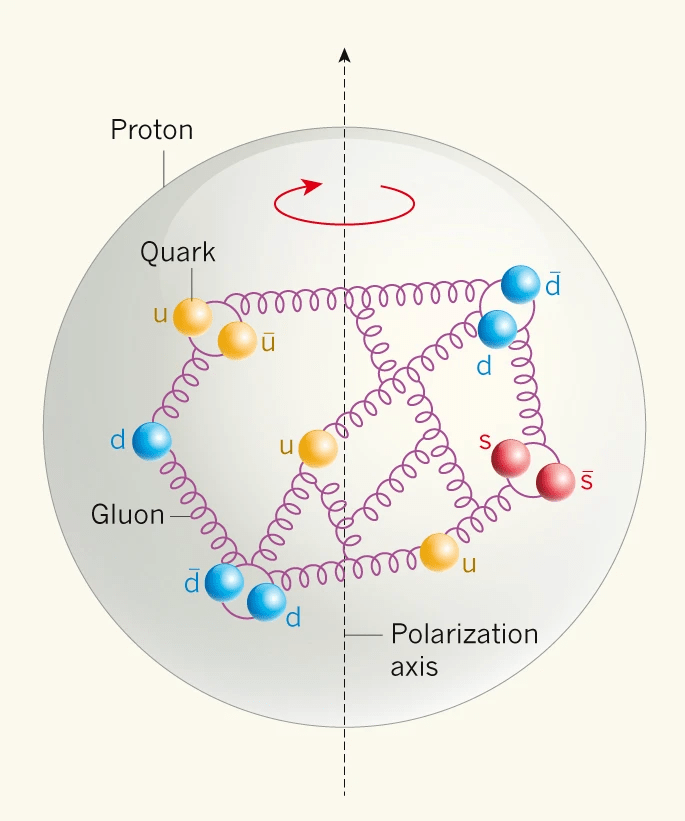
\includegraphics[width=0.4\textwidth]{C:/Users/Carmen/Desktop/Universidad/TFG/Borradores/img/proton.PNG}
	\caption[Estructura interna del protón]
	{Estructura interna de quarks del protón. \cite{protonYoung}}
	\label{fig:proton}
\end{figure}

El hallazgo del quark $s$ en el protón arroja luz sobre dos investigaciones actuales, principalmente. La primera tiene que ver con la $Q_{weak}$ o \textit{carga débil} del protón, la cual mide la  interacción débil entre el protón y el electrón y tiene como objetivo buscar una posible estructura interna de los quarks. El otro estudio que se beneficia del descubrimiento de la extrañeza y otros sabores ocultos en el protón, tiene que ver con la búsqueda de la materia oscura en el Universo. 


	\chapter{Interacción Débil}\label{cap:weak_int}
El origen de cada interacción fundamental se debe a causas diferentes. Por un lado, la existencia de carga eléctrica produce fuerzas electromagnéticas en las partículas y las hace interactuar entre sí, mientras que la interacción fuerte se debe a la propiedad del color, mencionada en el capítulo anterior. No todas las partículas tienen carga ni color simultáneamente por lo que no todas son susceptibles a las mismas interacciones. El caso de la interacción débil es bastante interesante porque muchas partículas con propiedades distintas son sensibles a ella. Por ejemplo, los leptones no tienen carga de color, no ``sienten'' la interacción fuerte, mientras los neutrinos no tienen carga eléctrica, por lo que no pueden interactuar mediante fuerzas electromagnéticas. Sin embargo, ambos tipos de partículas pueden estar presentes en interacciones débiles \cite{Griffiths2008}. Además, la causa de la interacción débil, aunque no tiene un nombre específico, suele denotarse como \textit{carga débil}.

Los mesones $\PK$ y muchas otras partículas decaen por interacción débil. Desde el principio se consideró un tratamiento cuántico-relativista para describir la fuerza débil y muchos científicos han contribuido al desarrollo de su formalismo. Cada interacción ocurre gracias al intercambio de una partícula mediadora o portadora de la fuerza de interacción. En la interacción fuerte es el gluón y en la electromagnética es el fotón. Las partículas mediadoras encargadas de transmitir la fuerza débil entre los quarks y leptones son los bosones vectoriales, llamados así por tener espín 1. Estos bosones, de gran masa, portadores de la interacción débil pueden estar cargados eléctricamente $\PWpm$ o ser neutros $\PZzero$. 

Hasta la década de los 70, sólo se habían observado procesos de intercambio de bosones cargados $\PWpm$. En los años 60 se empezó a formular una teoría que aunaba la interacción débil junto con la electromagnética, conocida hoy en día como \textit{Teoría Electrodébil}. Esta teoría predecía la existencia del bosón neutro mediador de la fuerza débil y dicha hipótesis fue confirmada experimentalmente en 1973 \cite{BrianM}, con el hallazgo de $\PZzero$.

Este capítulo se centra, principalmente, en la descripción de procesos de interacción débil con intercambio de bosones $\PWpm$ o procesos de \textit{interacción débil de corriente cargada} y nos servirá como base para el estudio del decaimiento de mesones $\PK$ cargados.

\section{Formalismo de la Interacción Débil}\label{cap:formalism}
La interacción débil se postula de forma análoga a la interacción electromagnética, la cual se basa en el acoplamiento del fotón con las corrientes electromagnéticas debidas a las cargas eléctricas en las partículas. Así, para la fuerza débil, se tienen corrientes débiles que se acoplan a los bosones vectoriales $\PWpm$ o $\PZzero$. De acuerdo con la Teoría Cuántica de Campos (TCC), cada partícula lleva asociado un campo cuántico $\phi(x)$, $\psi(x)$ o $W_{\mu}(x)$, dependiente del espacio y del tiempo $x^{\mu}=(ct,\boldsymbol{\vec{x}})$\protect\footnotemark. Estos campos actúan como operadores encargados de aniquilar partículas o crear antipartículas de espín $0$, $1/2 $ y $1$, respectivamente \cite{notas2020}. Para describir la evolución espacio-temporal de dichos campos asociados a partículas se hace uso de la densidad lagrangiana $\mathcal{L}$.

\footnotetext{Consultar el Apéndice \hyperref[cap:A]{A} para más información sobre la notación utilizada en este capítulo.}

Del mismo modo, las interacciones se describen mediante unas constantes, denominadas \textit{contantes de acoplamiento}, y productos entre los campos cuánticos de las partículas que intervienen en el proceso. Como $\mathcal{L}$ debe ser un escalar, sólo se permiten combinaciones entre campos que resulten en invariantes de Lorentz \cite{notas2020}. Esto es posible, ya que la TCC, entiende las interacciones como un intercambio de partículas mediadoras, tal y como se mencionó anteriormente. En su libro \cite{Bettini}, Bettini lo explica con el siguiente ejemplo: se tiene una partícula $a$ que interactúa en el campo mediado por el bosón $V$; en el vacío, $a$ está continuamente emitiendo y absorbiendo este bosón, tal y como se muestra en \ref{fig:bettini1}. No obstante, si una partícula $b$ se encuentra cerca de $a$ y tiene su misma interacción, puede absorber un bosón $V$ que previamente haya sido emitido por $a$ (ver \ref{fig:bettini2}). Entonces, se puede afirmar que $a$ y $b$ interactúan entre sí intercambiando un bosón $V$, es decir, combinando sus campos cuánticos mientras se crea y se aniquila $V$.
\begin{figure}[h]
\begin{subfigure}[t]{.5\textwidth}
  \centering
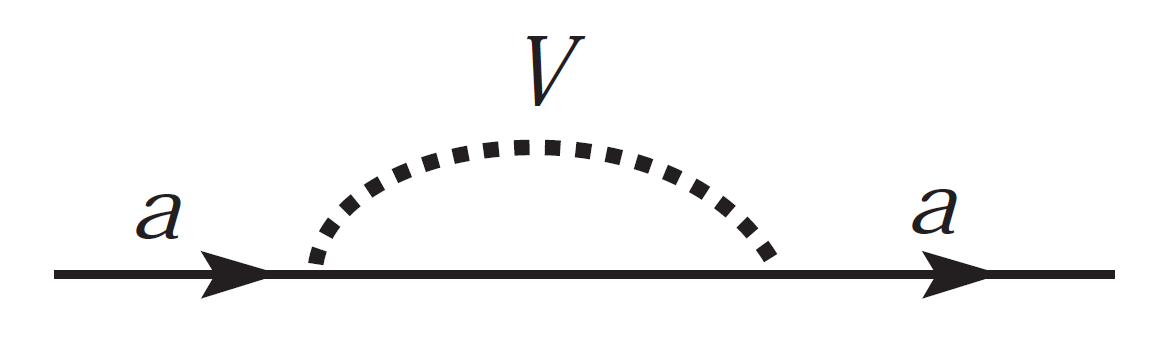
\includegraphics[width=0.6\linewidth]{{C:/Users/Carmen/Desktop/Universidad/TFG/Borradores/img/bettini1.PNG}}
\caption{$V$ emitido y reabsorbido por $a$}
  \label{fig:bettini1}
\end{subfigure}%
\begin{subfigure}[t]{.5\textwidth}
  \centering
  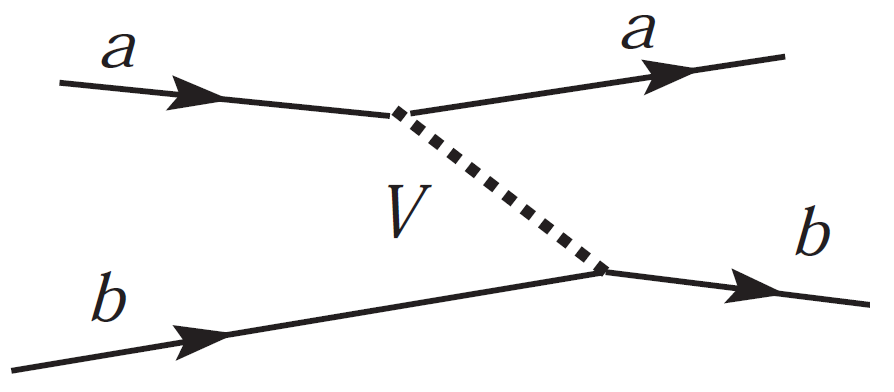
\includegraphics[width=0.6\linewidth]{{C:/Users/Carmen/Desktop/Universidad/TFG/Borradores/img/bettini2.PNG}}
  \caption{$V$ emitido por $a$ y absorbido por $b$}
  \label{fig:bettini2}
\end{subfigure}
\caption[Esquematización del proceso de interacción en TCC]{Proceso de interacción mediante intercambio del bosón mediador.  \cite{Bettini}}
\label{fig:bettini}
\end{figure}

Continuando con el ejemplo anterior, Bettini indica que el bosón mediador $V$ tiene, en general, una masa $m$ no nula, lo que provoca que, durante su emisión, se viole momentáneamente la conservación de energía $\Delta E = m$. Lo mismo, pero de forma opuesta ocurre durante su absorción. Así pues, la violación neta dura un $\Delta t$ y satisface la \textit{Relación de Indeterminación tiempo-energía}: $\Delta E \Delta t \leq \hbar$, lo que implica que $V$ sólo puede alejarse una distancia finita $R=c\Delta t$. Esta distancia equivale al rango de la fuerza de interacción, por lo tanto, cuanta mayor masa tenga el bosón mediador de una interacción, menor será su rango de alcance \cite{Bettini}. Dado que los bosones mediadores $\PWpm$ y $\PZzero$ tienen una masa muy grande ($m_W = \SI{80,379 \pm 0,012}{\GeV}$ y $m_Z = \SI{91,1876 \pm 0,0021}{\GeV}$, respectivamente \cite{Zyla}), la fuerza débil tiene un alcance muy corto, más que cualquier otra interacción fundamental, resultando en una intensidad muy tenue; de ahí la denominación de ``interacción débil''. 

Gráficamente, las interacciones se representan con Diagramas de Feynman. Estos diagramas proporcionan información acerca de la amplitud de probabilidad de los distintos procesos, donde cada línea representa a una partícula y cada vértice corresponde a cada actuación del lagrangiano de la interacción $\mathcal{L}$. La densidad lagrangiana $\mathcal{L}$ que describe cada vértice en el Diagrama de Feynman de una interacción de corriente cargada débil, tiene esta forma:
\begin{equation}
\mathcal{L}^{w}=\dfrac{g_{w}}{\sqrt{2}}\left( W^{\mu }\left( x\right) j_{\mu}^{+}\left( x\right) +\left[ W^{\mu }\left( x\right) \right]^{\ast }j_{\mu}^{-}\left( x\right) \right)\label{eq:weak_lagrangian}
\end{equation}

El campo $W^{\mu}(x)$ aniquila $\PWp$ o crea $\PWm$ mientras que su conjugado $\left(W^{\mu}(x)\right)^\ast$ aniquila $\PWm$ o crea $\PWp$. En un proceso que ocurre por interacción débil con intercambio de $\PWpm$, la carga neta del estado inicial y el final difieren en una unidad y, entonces, se habla de interacción de corriente cargada. Luego, la densidad de corriente débil $j_{\mu}$ puede ser positiva o negativa, y se compone de dos términos, uno para la corriente leptónica y otro para la hadrónica:
\begin{equation}
j_{\mu} ^{\pm }\left( x\right) =j_{\mu} ^{\pm lep}\left( x\right) +j_{\mu} ^{\pm had}\left( x\right) \label{eq:weak_current_hadylep}
\end{equation}
La corriente leptónica es una composición de corrientes de cada familia de leptones, así se tiene un término para los electrones, otro para los muones y otro para los taones:
\begin{equation}
j_{\mu }^{\pm lep}\left( x\right) =j_{\mu }^{\pm el}\left( x\right) +j_{\mu }^{\pm muon}\left( x\right) +j_{\mu} ^{\pm tau}\left( x\right)\label{eq:leptonic_weak_current}
\end{equation}
La corriente leptónica de electrones puede expresarse de la siguiente forma:
\begin{align}
j_{\mu }^{-el}\left(x\right)&=i\overline{\psi}_{e}\left( x\right) \dfrac{1-\gamma_{5}}{2}\gamma _{\mu }\psi_{{ \nu}_{e}}\left( x\right) & j_{\mu}^{+el}\left(x\right)&= i\overline{\psi}_{{\nu}_{e}}\left(x\right) \dfrac{1-\gamma_{5}}{2}\gamma _{\mu}\psi_{e}\left( x\right)\label{eq:electric_weak_current}
\end{align}
La corriente negativa $j_{\mu }^{-el}$, aniquila $\nu_e$ (o crea $\overline{\nu_e}$) y crea $e^-$ (o aniquila $e^+$), mientras que la corriente positiva $j_{\mu }^{+el}$ hace justo lo opuesto. $j_{\mu }^{\pm muon}$ y $j_{\mu }^{\pm tau}$ pueden definirse de manera análoga. Estas corrientes leptónicas se caracterizan por conservar el número cuántico leptónico y la carga de las partículas que intervienen. 

El operador de corriente hadrónica $j_{\mu} ^{\pm had}$ es el encargado de crear o aniquilar hadrones, conservando siempre el número bariónico $B$ e incrementando o reduciendo en una unidad la carga eléctrica total $Q$. Sin embargo, aunque no siempre, también son capaces de modificar la extrañeza: la corriente hadrónica positiva (negativa) puede aumentar (disminuir) la extrañeza en una unidad $\Delta S = +1$ ($\Delta S = -1$) \cite{notas2020}.

Además, $g_W$ es la constante de acoplo de la interacción débil y se relaciona con la constante de Fermi $G_F$ según \ref{eq:fermi_coupling}. Experimentalmente se ha comprobado que $G_F$ tiene un valor único para todos los procesos donde interviene la interacción débil, siendo este $G_{F}= \SI{1,166e-5}{\per\GeV\squared}$.
\begin{equation}
\dfrac{G_{F}}{{g_{w}}^2}=\dfrac{\sqrt{2}}{8{m_{W}}^2}\label{eq:fermi_coupling}
\end{equation}

Si se reescribe la corriente débil leptónica de la ecuación \ref{eq:electric_weak_current} en su forma expandida, pueden distinguirse dos términos:
\begin{equation}
j_{\mu}^{+el}\left(x\right)= \dfrac{i}{2} \{ \overline{\psi}_{{\nu}_{e}}\left(x\right)\gamma _{\mu}\psi_{e}\left( x\right)- \overline{\psi}_{{\nu}_{e}}\left(x\right)\gamma _{\mu}\gamma_{5}\psi_{e}\left( x\right) \}
\end{equation}
El primero $\overline{\psi}_{{\nu}_{e}}\gamma _{\mu}\psi_{e}$ se transforma como un vector polar (V) y el segundo término $\overline{\psi}_{{\nu}_{e}}\gamma _{\mu}\gamma_{5}\psi_{e}$ como un vector axial (A). Debido a esto, la corriente débil se dice que tiene estructura V-A. Esta estructura no es exclusiva para la corriente débil leptónica, sino que también está presente en la corriente débil hadrónica, salvo alguna constante de acoplamiento. 

Inicialmente, se introdujo la parte correspondiente al vector polar en la corriente débil por analogía con la interacción electromagnética. El término del vector axial fue añadido posteriormente, tras el descubrimiento de la violación de paridad \cite{Paschos}. Si una interacción presenta la estructura anterior de Vector polar - vector Axial, se dice que es una \textit{Interacción V-A}.

Por lo tanto, el lagrangiano $\mathcal{L}$ de una interacción débil presentar estructura V-A o, en su forma más general, una combinación o producto de estructuras V-A \cite{Renton}, una para describir el decaimiento de los leptones y otra para los quarks:
\begin{equation}
\mathcal{L}= \sum _{i} C_{i}\left(\overline{\psi}_{\nu_l}\widehat{\Gamma_{i}}\psi _{l}\right)\left( \overline{\psi }_{q_2}\widehat{\Gamma^{i}}\psi _{q_1}\right)
\end{equation}
Los coeficientes $C_i$ son constantes de acoplamiento del proceso en cuestión y los $\psi_i$ son los bi-espinores resultantes de la ecuación de Dirac que describe cada fermión (quark o lepton) que participa en la interacción. Los $\widehat{\Gamma_{i}}$ son covariantes bilineales, los cuales proporcionan información sobre cómo se transforman dichas partículas (ver Apéndice \hyperref[cap:A]{A}).

A la hora de analizar el decaimiento de mesones $\PK$, la magnitud que más interesa calcular es la probabilidad de decaimiento $\Gamma$. $\Gamma$ indica la probabilidad por unidad de tiempo de que el kaón (o cualquier partícula) sufra un proceso de desintegración. Por ejemplo, si se tiene un conjunto de partículas $N(t)$ en un instante $t$, una porción $N\Gamma dt$ de ellas decaerá en el próximo instante $dt$ \cite{Griffiths2008}:
\begin{align}
dN &= -\Gamma Ndt & N(t) &= N(0)e^{-\Gamma t}
\end{align}
Además, esta magnitud $\Gamma$ está relacionada con la semivida de la partícula $\tau$:
\begin{equation}
\tau=\dfrac{1}{\Gamma}\label{eq:meanlife}
\end{equation}
Como, en general, las partículas pueden decaer de distintas formas o modos:
\begin{align}
\Gamma_{total} &= \sum_{i=1}^N \Gamma_i & \tau=\dfrac{1}{\Gamma_{total}}
\end{align}
Por este motivo, también es posible definir el ratio de desintegración o branching ratio ($BR$) para un modo de decaimiento $i$ dado:
\begin{equation}
BR(i)=\dfrac{\Gamma_{i}}{\Gamma_{total}}
\end{equation}

En unidades naturales ($\hbar=c=1$), la probabilidad de decaimiento $\Gamma$ es:
\begin{equation}
2\pi \left| \mathcal{M}\right| ^{2} \rho\left( E\right)
\end{equation} 
Siendo $\mathcal{M}$ la amplitud de probabilidad y $\rho\left(E\right) \equiv \rho$ la densidad de estados finales del proceso.

Por un lado, la densidad de estados finales (o espacio de fases) depende de las masas, las energías y los momentos de las partículas que intervienen en el decaimiento, es decir, contiene toda la información cinemática del proceso. Por otra parte, la amplitud de probabilidad (también conocida como elemento de matriz) es una magnitud que está relacionada con el lagrangiano de la interacción $\mathcal{L}$ y, por lo tanto, proporciona información acerca de la dinámica del decaimiento. 

Los mesones $\PK$ son partículas de espín 0, por lo que el campo escalar que los describe satisface la ecuación de Klein-Gordon, que en forma covariante tiene la siguiente expresión:
\begin{equation}
\left( \square +m^{2}\right) \psi \left( x\right) =0
\end{equation}

Además, la densidad lagrangiana ${\mathcal{L}}^w$ que describe el decaimiento de los mesones $\PK$ por interacción débil es invariante de Lorentz, por lo que se cumple que \cite{Halzen}
\begin{equation}
\mathcal{M}=-i \int {\mathcal{L}}^w \left(x\right) d^{4}x \propto -i\int j_{\mu }W^{\mu }d^{4}x
\end{equation}

Para hallar $d\Gamma$, se hace uso de la \textit{Regla de Oro de Fermi} para procesos de desintegración del tipo $1 \rightarrow 2+3$:
\begin{equation}
d\Gamma =\left| \mathcal{M}\right| ^{2}\dfrac{S}{2m_{1}}\left[ \left( \dfrac{d^{3}\boldsymbol{p}_{2}}{\left( 2\pi \right) ^{3}2E_{2}}\right) \left( \dfrac{d^{3}\boldsymbol{p}_{3}}{\left( 2\pi \right) ^{3}2E_{3}}\right) \right] \times \left( 2\pi \right) ^{4}\delta ^{4}\left( p_{1}-p_{2}-p_{3}\right) 
\end{equation}

Los diagramas de Feynman son una herramienta muy útil a la hora de calcular de forma rápida y sencilla $\left| \mathcal{M}\right|$. Para ello, sólo debemos de seguir las reglas del cálculo de Feynman en unidades naturales \cite{Griffiths2008}:

\begin{enumerate}
\item \underline{Notación}: Etiquetar todos los cuadri-momentos (internos y externos) del proceso y asignar flechas a cada línea.
\item \underline{Líneas externas}: Para partículas y antipartículas llegando al vértice escribir los espinores $u$ y $\overline{v}$, respectivamente. Si salen del vértice, entonces se escribe: $\overline{u}$ y $v$, en cada caso.
\item \underline{Factor de vértice}: Para cada vértice, escribir un factor $\dfrac{-ig_{w}}{2\sqrt{2}}\gamma ^{\mu }\left( 1-\gamma ^{5}\right)$. 
\item \underline{Propagadores}: Para cada línea interna que represente un bosón vectorial $\PWpm$ o $\PZzero$, escribir un factor: 
$\dfrac{-i\left( g_{\mu\nu }-q_{\mu }q_{\nu }/M^{2}\right) }{q^{2}-M^{2}}$. Pero, en general, como $q^{2}\ll \left( M\right)^{2}$ puede realizarse la siguiente aproximación para describir el vértice: $\dfrac{ig_{\mu \nu }}{\left( M\right) ^{2}}$.
\item \underline{Conservación de momento y energía}: Para cada vértice, escribir $\left( 2\pi \right) ^{4}\delta ^{4}\left( k_{1}+k_{2}+k_{3}\right)$. En esta expresión $k$ es el vector momento de 3 componentes dirigiéndose hacia el vértice. Si el momento sale del vértice entonces lleva un signo menos.
\item \underline{Integrar sobre todos los momentos}: Para cada cuadri-momento $q$, escribir un factor $\dfrac{d^{4}q}{\left( 2\pi \right) ^{4}}$ e integrar.
\item \underline{Cancelar la función Delta $\Delta$}: Cancelar el factor restante $\left( 2\pi \right) ^{4}\delta ^{4}\left( p_{1}+p_{2}+\ldots -p_{n}\right)$ e igualar la expresión resultante a $-i\mathcal{M}$.
\end{enumerate}


\subsection{Interacción débil en el Modelo de Quarks}\label{sec:weak_int_quarks}
En el modelo de Quarks, la interacción débil se describe mediante Diagramas de Feynman, donde se produce un cambio de sabor en los quarks, emitiendo bosones $\PWpm$. Como consecuencia de la conservación del número leptónico en esta interacción, el acoplamiento de $\PWpm$ ocurre de manera estricta entre leptones de la misma generación \cite{Griffiths2008}: 
\begin{align}
\begingroup 
\renewcommand*{\arraystretch}{0.8}
\setlength\arraycolsep{10pt}
\begin{pmatrix} \nu _{e} \\ e \end{pmatrix} \qquad
\begin{pmatrix} \nu_{\mu } \\ \mu \end{pmatrix} \qquad
\begin{pmatrix} \nu_{\tau} \\ \tau \end{pmatrix}
\endgroup
\end{align}
No obstante, $W^{\pm}$ sí puede acoplarse a quarks de distintas generaciones:
\begin{align}
\begingroup 
\renewcommand*{\arraystretch}{0.8}
\setlength\arraycolsep{10pt}
\begin{pmatrix} u \\ d \end{pmatrix} \qquad
\begin{pmatrix} c \\ s \end{pmatrix} \qquad
\begin{pmatrix} t \\ b \end{pmatrix}
\endgroup
\end{align}

Cuando únicamente se habían descubierto los quarks ligeros, en torno a 1963, Cabibbo sugirió que este acoplamiento inter-generacional como explicación al fenómeno de violación de la extrañeza en la interacción débil. Así, en un Diagrama de Feynman, la corriente hadrónica débil mantiene la estructura V-A, pero su expresión puede variar dependiendo de si se conserva o no la extrañeza en el vértice a estudio del proceso:
\begin{itemize}
\item Sin cambio de extrañeza, se aniquila un quark $\Pqd$ y se crea un quark $\Pqu$: $\Pqd \rightarrow \Pqu + \PWm$
\end{itemize}
\begin{equation}
j_{\mu}^{+had}(\Delta S= 0)=\cos \left( \theta _{c}\right) i\overline{\psi }_{u}\left( x\right) \dfrac{1-\gamma _{5}}{2}\gamma _{\mu }\psi _{d}
\end{equation}
\begin{itemize}
\item Con cambio de extrañeza, se aniquila un quark $s$ y se crea un quark $\Pqu$: $\Pqs \rightarrow \Pqu + \PWm$
\end{itemize}
\begin{equation}
j_{\mu}^{+had}(\Delta S= 0)=\sin \left( \theta _{C}\right) i\overline{\psi }_{u}\left( x\right) \dfrac{1-\gamma _{5}}{2}\gamma _{\mu }\psi _{s}
\end{equation}
donde $\theta_{C}$ hace referencia al ángulo de Cabibbo, cuyo valor experimental ha resultado ser $13,02\degree$.

La teoría de Cabibbo era bastante acertada al dar explicación a numerosos decaimientos de quarks. Sin embargo, esta teoría también permitía el decaimiento del mesón $\PKz$ en $\APmuon\Pmuon$, cuya amplitud de probabilidad era proporcional a $\cos \left( \theta _{C}\right) \sin \left( \theta _{C}\right)$ y, por lo tanto, mucho mayor que la obtenida experimentalmente.  Para solucionar esta contradicción, en 1970, Glashow, Iliopoulos y Maiani (GIM), propusieron la existencia de un nuevo quark $\Pqc$ que debía acoplarse con $-\Pqd \cdot \sin \left( \theta _{C}\right) + \Pqs \cdot \cos \left( \theta_C \right)$, la combinación ortogonal a $\Pqd \cdot \cos \left( \theta _{C}\right) + \Pqs \cdot \sin \left( \theta _{C}\right)$, a la que se acoplaba el sabor $\Pqu$ \cite{Griffiths2008}.

Nacía así, la teoría Cabibbo-GIM, la cual afirmaba que los estados de los quarks $\Pqd$ y $\Pqs$, en lugar de su descripción física, debían definirse como:
\begin{equation}
\begin{gathered}
\Pqd'=\Pqd \cdot \cos \left( \theta _{C}\right) + \Pqs \cdot \sin \left( \theta _{C}\right) \\
\Pqs'= - \Pqd \cdot \sin \left( \theta _{C}\right) + \Pqs \cdot \cos \left( \theta_C\right)
\end{gathered}
\end{equation}
De manera que los $\PWpm$ se acoplaran a las familias de quarks como hacían los leptones, pero con la definición correcta de los estados de los quarks o quarks \textit{rotados}:
\begin{align}
\begingroup 
\renewcommand*{\arraystretch}{0.8}
\setlength\arraycolsep{10pt}
\begin{pmatrix} \Pqu \\ \Pqd' \end{pmatrix} \qquad
\begin{pmatrix} \Pqc \\ \Pqs' \end{pmatrix}
\endgroup
\end{align}

En 1973, Kobayashi y Maskawa, en un intento de dar explicación a la violación CP, generalizaron el esquema de Cabibbo-GIM, para incluir una tercera generación de quarks, aún sin descubrir en aquel entonces, surgiendo así la \textit{matriz CKM} (Cabibbo-Kobayashi-Maskawa):
\begin{equation}
\begingroup 
\renewcommand*{\arraystretch}{0.8}
\setlength\arraycolsep{10pt}
\begin{pmatrix} \Pqd' \\ \Pqs' \\ \Pqb' \end{pmatrix} =\begin{pmatrix} V_{ud} & V_{us} & V_{ub} \\ V_{cd} & V_{cs} & V_{cb} \\ V_{td} & V_{ts} & V_{tb} \end{pmatrix}\begin{pmatrix} d \\ s \\ b \end{pmatrix}
\endgroup\label{eq:CKM}
\end{equation}

Esta matriz permitía conectar todos los sabores de quarks entre sí, siendo los elementos de su diagonal los más importantes, al relacionar quarks de la misma familia: $\Pqu \leftrightarrow \Pqd$, $\Pqc \leftrightarrow \Pqs$ y $\Pqt \leftrightarrow \Pqb$. En definitiva, proporciona información acerca de la probabilidad de transición de un quark $i$ a un quark $j$. Los términos no diagonales son los responsables de que los quarks pesados vayan decayendo progresivamente en los sabores ligeros $\Pqu$ y $\Pqd$, que son los constituyentes predominantes de la materia ordinaria. Así, por ejemplo, $V_{ud}$ describe el acoplamiento de $\Pqu$ a $\Pqd$: $\Pqd \rightarrow \Pqu + \PWm$.

La matriz CKM puede reducirse a una especie de ``forma canónica'' utilizando los \textit{ángulos generalizados de Cabibbo} $\theta_{1}$, $\theta_{2}$, $\theta_{3}$, y un factor de fase $e^{i\delta}$ \cite{Griffiths2008}:
\begin{equation}
\begingroup 
\renewcommand*{\arraystretch}{0.8}
\setlength\arraycolsep{10pt}
|V|=
\begin{pmatrix} c_{1} & s_{1}c_{3} & s_{1}s_{3} \\ -s_{1}c_{2} & c_{1}c_{2}c_{3}-s_{2}s_{3}e^{i\delta } & c_{1}c_{2}s_{3}+s_{2}c_{3}e^{i\delta } \\ -s_{1}s_{2} & c_{1}s_{2}c_{3}+c_{2}s_{3}e^{i\delta } & c_{1}s_{2}s_{3}-c_{2}c_{3}e^{i\delta } \end{pmatrix}
\endgroup
\end{equation}

con $c_{i}\equiv \cos \theta _{i}$ y $s_{i}\equiv \sin \theta _{i}$.

Si $\theta _{2}=\theta _{3}=0$, entonces $\theta _{1}=\theta _{C}$, obteniéndose la representación Cabibbo-GIM anterior. Los elementos $|V_{ij}|$ de la matriz CKM suelen determinarse empíricamente, pero en concreto, el promedio de $|V_{ud}|$ y el de $|V_{us}|$ se conocen con bastante exactitud.\\

\section{Decaimiento de mesones $K$ cargados}
\label{sec:charged_kaon_decay}
Los mesones $\PKpm$ decaen por interacción débil y sus procesos de decaimiento (modos) pueden clasificarse en varias categorías. A continuación, presentamos los modos leptónicos, semileptónicos y hadrónicos, que son los más relevantes:

\begin{table}[!htb]
\begin{minipage}{.5\linewidth}
    \centering
\begin{tabular}{ c c } 
\toprule
\makecell{Mesón $\PKp$}  &  Mesón $\PKm$ \\
\midrule   
$\Pep\Pnu_{e}$ & $\Pem\APnu_{e}$ \\
$\APmuon\Pnu_{\mu}$ & $\Pmuon\APnu_{\mu}$ \\
$\Pgpz\Pep\Pnu_{e}$ & $\Pgpz\Pem\APnu_{e}$ \\
$\Pgpz\APmuon\Pnu_{\mu}$ & $\Pgpz\Pmuon\APnu_{\mu}$ \\
$\Pgpz\Pgpz\Pep\Pnu_{e}$ & $\Pgpz\Pgpz\Pem\APnu_{e}$ \\
$\Pgpp\Pgpm\Pep\Pnu_{e}$ & $\Pgpp\Pgpm\Pem\APnu_{e}$ \\
$\Pgpp\Pgpm\APmuon\Pnu_{\mu}$ & $\Pgpp\Pgpm\Pmuon\APnu_{\mu}$ \\
$\Pgpz\Pgpz\Pgpz\Pep\Pnu_{e}$ & $\Pgpz\Pgpz\Pgpz \Pem \APnu_{e}$ \\
\bottomrule
\end{tabular}
\caption[Modos de decaimiento leptónicos y semileptónicos de $\PKpm$]{Modos (semi-)leptónicos. \cite{Zyla}}
\label{tab:Kpm_leptonic_decay}
\end{minipage}\hfill
\begin{minipage}{.5\linewidth}
    \centering
\begin{tabular}{ c c } 
    \toprule
    \makecell{Mesón $\PKp$}  &  Mesón $\PKm$ \\    
    \midrule
$\Pgpp\Pgpz$ & $\Pgpm\Pgpz$ \\
$\Pgpp\Pgpz\Pgpz$ & $\Pgpm\Pgpz\Pgpz$ \\
$\Pgpp\Pgpp\Pgpm$ & $\Pgpp\Pgpm\Pgpm$ \\
    \bottomrule
\end{tabular}
\caption[Modos de decaimiento hadrónicos de $\PKpm$]{Modos hadrónicos. \cite{Zyla}}
\label{tab:Kpm_hadronic_decay}
\end{minipage}
\end{table}

Como puede observarse, los modos de decaimiento de $\PKm$ son los mismos modos que los de $\PKp$ pero con carga conjugada. Sin embargo, no todos estos procesos tienen la misma probabilidad de ocurrir. Como ejemplo ilustrativo de esta afirmación, centramos el estudio en los modos leptónicos del mesón $\PKm$: $\PKm \rightarrow \Pem \APnu_{e}$ y $\PKm \rightarrow \Pmuon \APnu_{\mu}$.

El Diagrama de Feynman de quarks de $\PKm \rightarrow \Plm + \Pagnl$ aparece en la figura \ref{fig:diagrama1}.

\begin{figure}[ht!]
	\centering
	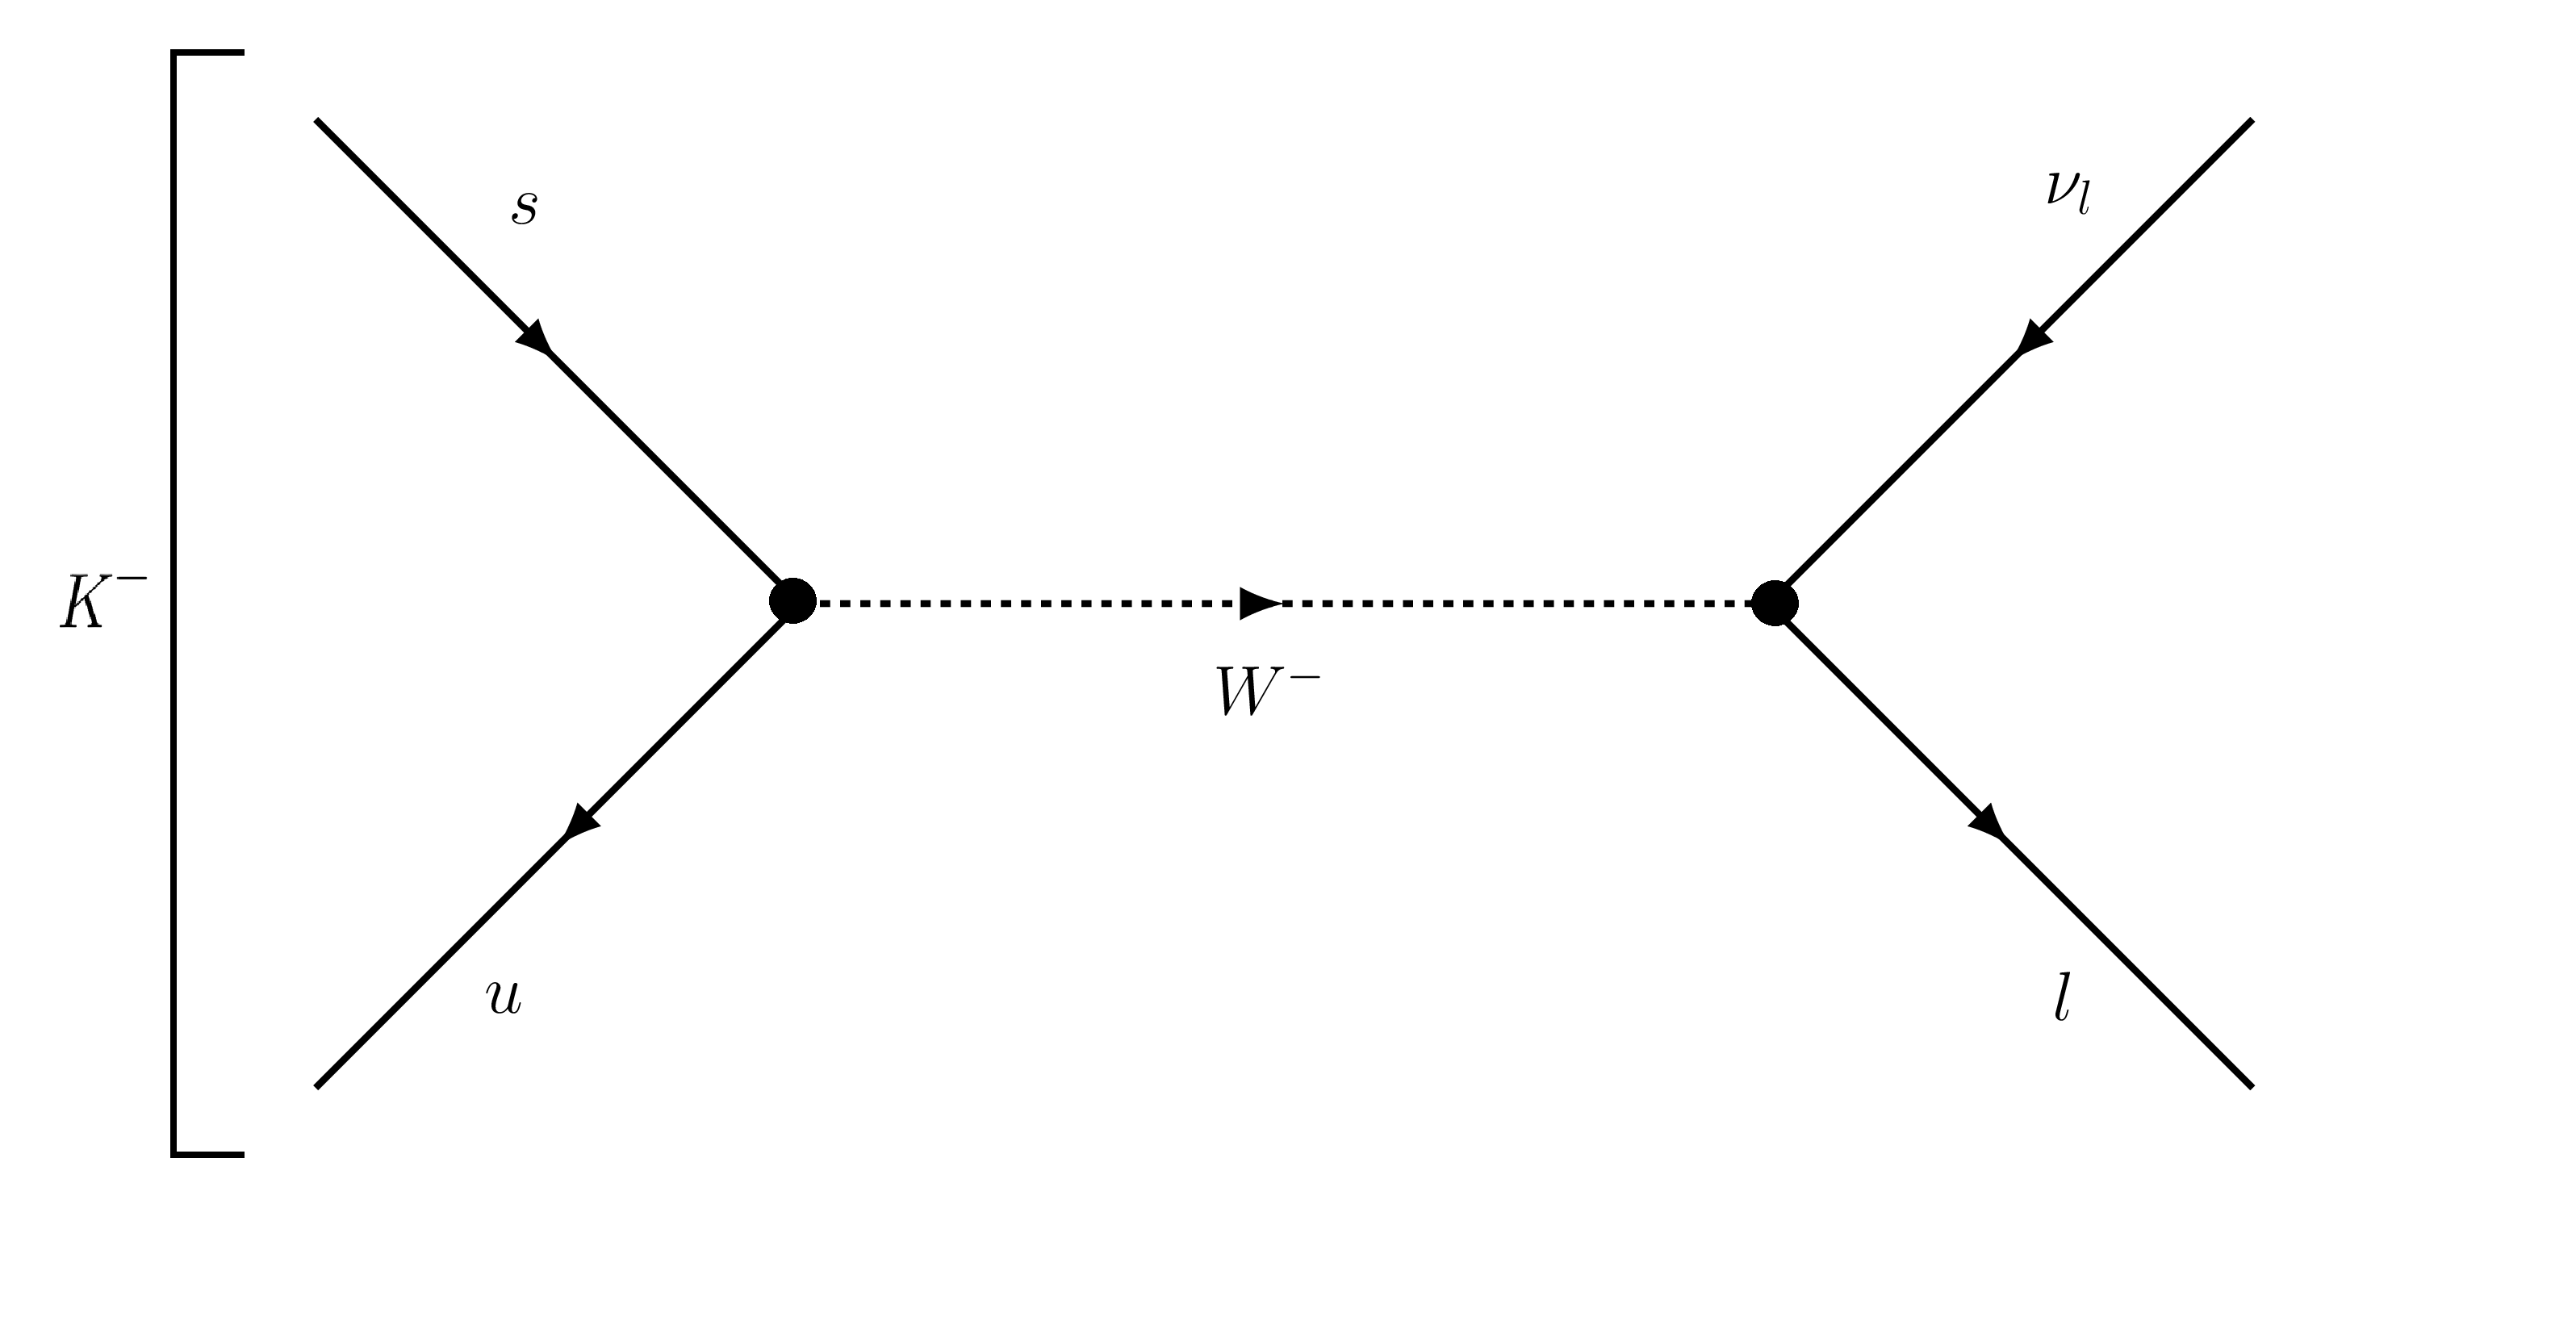
\includegraphics[width=0.95\textwidth]{C:/Users/Carmen/Desktop/Universidad/TFG/Borradores/img/kaon1.png}
	\caption[Diagrama de Feynman de quarks de $\PKm \rightarrow \Plm + \Pagnl$]
	{Diagrama de Feynman del modo leptónico de $\PKm$ en el Modelo de Quarks.}
	\label{fig:diagrama1}
\end{figure}

El vértice leptónico está totalmente definido a partir de las expresiones de corriente débil vistas en el formalismo anterior. Sin embargo, el vértice hadrónico es algo más complejo de explicar y puede hacerse mediante dos enfoques. El primero de ellos consiste en una descripción a partir de la composición de quarks de $\PKm$, pero este tratamiento presenta una dificultad de cálculo y formalismo teórico demasiado avanzado. Por ello, y dado que el mesón $\PK$ es una partícula de espín 0, resulta más sencillo describir dicho vértice hadrónico a partir de la ecuación de Klein-Gordon.

Siguiendo este segundo procedimiento, redibujamos el diagrama $\PKm \rightarrow \Plm + \Pagnl$ como se ve en la figura \ref{fig:diagrama2}, donde también se han etiquetado los momentos internos y externos de cada partícula que interviene. El punto gordo que se aprecia en el vértice hadrónico, simplemente indica que, como el mesón $\PKm$ posee una estructura interna más elemental de quarks, no sabemos de antemano cómo interacciona con el propagador $\PWm$. Por ello, para el vértice hadrónico se escribe un factor: $\dfrac{-ig_{w}}{2\sqrt{2}}F^{\mu}$. El término $F^{\mu}$ se conoce como \textit{factor de forma}; es un cuadrivector dependiente del momento del mesón $\PKm$ que describe la interacción en el vértice hadrónico con el propagador.

\begin{figure}[ht!]
	\centering
	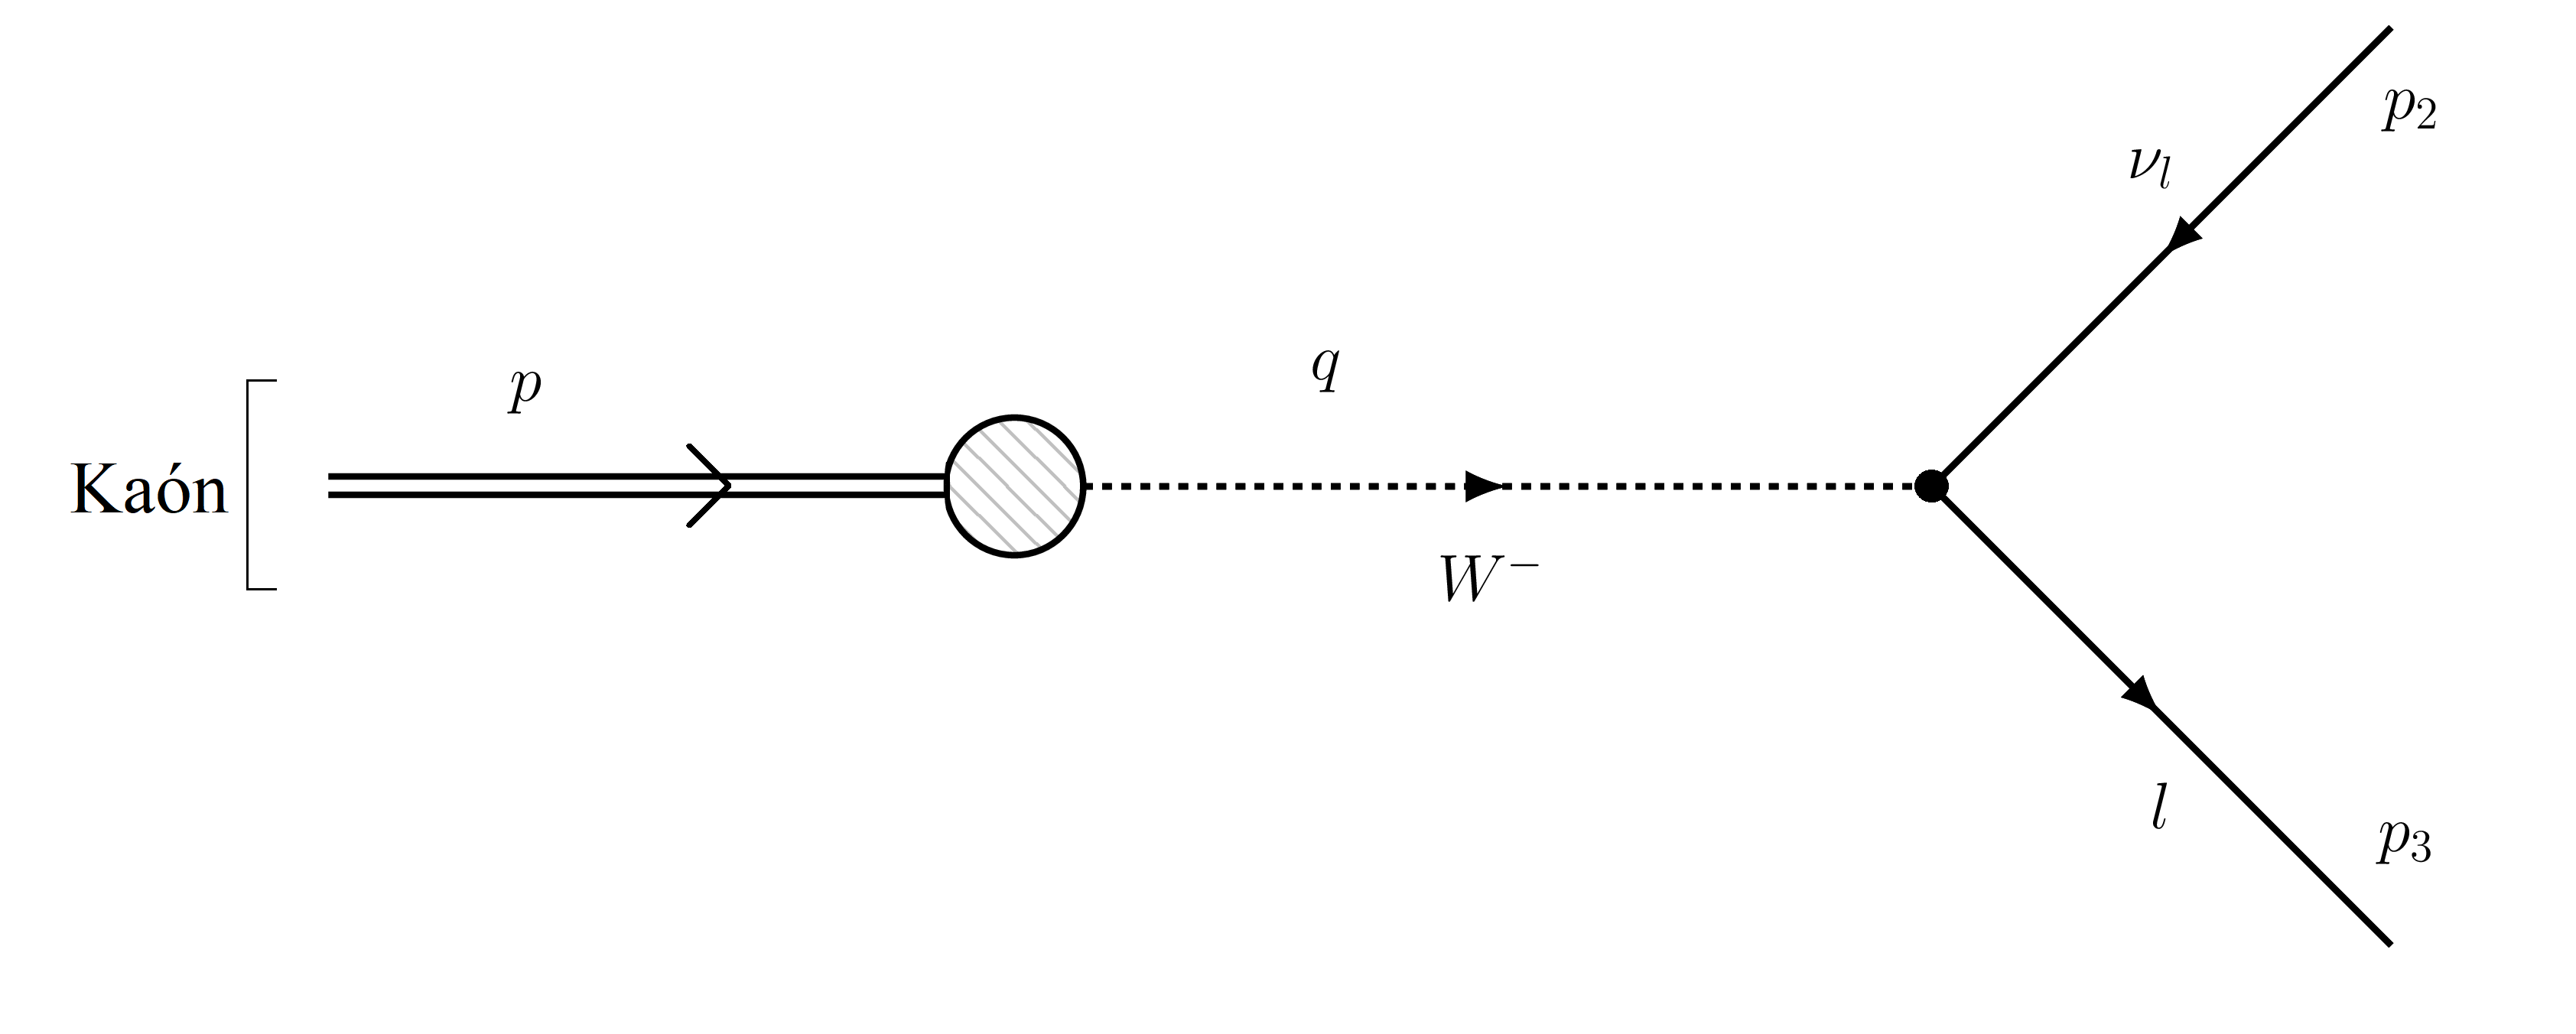
\includegraphics[width=0.95\textwidth]{C:/Users/Carmen/Desktop/Universidad/TFG/Borradores/img/kaon2.png}
	\caption[Diagrama de Feynman de $\PKm \rightarrow \Plm + \Pagnl$ con los momentos]
	{Diagrama de Feynman de $\PKm \rightarrow \Plm + \Pagnl$ con los momentos de cada partícula.}
	\label{fig:diagrama2}
\end{figure}

Analizamos el diagrama de la figura \ref{fig:diagrama2} y aplicamos las reglas de Feynman para calcular la amplitud de decaimiento del proceso, con el objetivo de hallar la probabilidad de que ocurran tales modos de decaimiento. 

Así se obtiene que:
\begin{equation}
\mathcal{M} =\dfrac{{g_{w}}^2}{8\left( M_W\right)^{2}}\left[ \overline{u}\left(3\right) \gamma_{\mu}\left( 1-\gamma^{5} \right) v\left( 2\right) \right] F^{\mu}\label{eq:Msimple}
\end{equation}
con $F^{\mu}=f_K p^{\mu}$, siendo $f_K$ la constante de decaimiento del kaón; desconocida en principio.

Aplicando el truco de Casimir (ver eq. \ref{eq:casimir_trick}) y haciendo la media, se llega a la siguiente expresión:
\begin{equation}
\left\langle |\mathcal{M}|^{2}\right\rangle=\dfrac{1}{8}\left[ f_{K}\left( \dfrac{g_w}{M_W}\right) ^{2}\right] ^{2}\left[2\left( p\cdot p_{2}\right) \left( p\cdot p_{3}\right) -p^{2}\left( p_{2}\cdot p_{3}\right)\right]\label{eq:amplitudM}
\end{equation}

Teniendo en cuenta que $p=p_{2}+p_{3}$ junto con $p^2={m_K}^2$ y ${p_3}^2={m_{\Pl}}^2$, y sabiendo que el antineutrino carece de masa: ${p_2}^2={m_{\nu}}^2=0$, reescribimos:
\begin{align}
p\cdot p_{2} &= p_{3} \cdot p_{2} & p \cdot p_{3} &= p_{2} \cdot p_{3}+{m_{\Pl}}^2
\end{align}

Además,
\begin{equation}
p^{2}={p_{2}}^{2}+{p_3}^{2}+2\left( p_{2} \cdot p_{3}\right) \longrightarrow 2\left( p_{2} \cdot p_{3}\right)=\left( m_{K}^{2}-m_{\Pl}^{2}\right)
\end{equation}

Sustituyendo en la ecuación \ref{eq:amplitudM}, se llega a:
\begin{equation}
\left\langle |\mathcal{M}|^{2}\right\rangle=\left( \dfrac{g_w}{2M_W}\right)^{4} {f_K}^2 {m_{\Pl}}^{2}\left( {m_{K}}^{2}-{m_{\Pl}}^{2}\right)\label{eq:amplitudmedia}
\end{equation}

Así, la expresión final para la probabilidad del decaimiento leptónico de $\PKm$ es:
\begin{equation}
\Gamma =\dfrac{{f_{K}}^{2}}{\pi {m_{K}}^{3}}\left( \dfrac{g_w}{4M_W}\right)^{4}{m_{\Pl}}^{2}\left({m_{K}}^{2}-{m_{\Pl}}^{2}\right)^{2}\label{eq:decayrate}
\end{equation}

Para ver un desarrollo detallado paso a paso de cómo se obtienen las ecuaciones \ref{eq:Msimple}, \ref{eq:amplitudM}, \ref{eq:amplitudmedia} y \ref{eq:decayrate}, consultar el Apéndice \hyperref[cap:B]{B}.

Comparando los dos modos de decaimiento posibles $\PKm \rightarrow \Pem \APnu_{e}$ y $\PKm \rightarrow \Pmuon \APnu_{\mu}$:
\begin{equation}
\dfrac{\Gamma \left( \PKm \rightarrow \Pem \APnu_{e}\right) }{\Gamma \left( \PKm \rightarrow \Pmuon \APnu_{\mu}\right) }=\dfrac{m_{e}^{2}\left( m_{K}^{2}-m_{e}^{2}\right) ^{2}}{m_{\mu }^{2}\left( m_{K}^{2}-m_{\mu }^{2}\right) ^{2}}=\dfrac{\left( 0,511\right) ^{2}\left( 493,677^{2}-0,511^{2}\right) ^{2}}{\left( 105,7\right) ^{2}\left( 493,677^{2}-105,7^{2}\right) ^{2}}=\num{2,57e-5}\label{eq:BRkaon}
\end{equation}

Las masas anteriores tienen unidades de MeV. Si procedemos de forma análoga para el pión $\Pgp$, se tiene que:
\begin{equation}
\dfrac{\Gamma \left( \Pgpm \rightarrow \Pem \APnu_{e}\right) }{\Gamma \left( \Pgpm \rightarrow \Pmuon \APnu_{\mu}\right) }=\dfrac{m_{e}^{2}\left( m_{\pi}^{2}-m_{e}^{2}\right) ^{2}}{m_{\mu }^{2}\left( m_{\pi}^{2}-m_{\mu }^{2}\right) ^{2}}=\dfrac{\left( 0,511\right) ^{2}\left(139,57^{2}-0,511^{2}\right) ^{2}}{\left( 105,7\right) ^{2}\left( 139,57^{2}-105,7^{2}\right) ^{2}}=\num{1,28e-4}\label{eq:BRpion}
\end{equation}

Estos valores de las ratios son muy parecidos a los datos experimentales \cite{tanabashi} \cite{olive}:
\begin{align}
\dfrac{\Gamma \left( \PKm \rightarrow \Pem \APnu_{e}\right)}{\Gamma \left( \PKm \rightarrow \Pmuon \APnu_{\mu}\right)} &= \num{2,488(09)e-5} & \dfrac{\Gamma \left( \Pgpm \rightarrow \Pem \APnu_{e}\right)}{\Gamma \left( \Pgpm \rightarrow \Pmuon \APnu_{\mu}\right)} &= \num{1,230(04)e-4}\label{eq:BRexp}
\end{align}

El resultado de las dos ratios indica que, tanto el pión como el mesón $\PK$, prefieren el modo leptónico del $\Pmuon$ sobre el $\Pem$. En un principio, este hecho puede parecer sorprendente puesto que la masa del muón es mucho mayor que la del electrón y, de acuerdo con las consideraciones de la densidad de estados finales, se favorecen los decaimientos con la disminución de masa más grande. Esto quiere decir que, excluyendo aquellos casos donde intervenga alguna ley de conservación, el estado final de las desintegraciones suele ser el más ligero. 

Los modos leptónicos de $\PK$ y $\Pgp$ suponen una excepción a esta norma. Este hecho puede entenderse teniendo en cuenta que, tanto el pión como el kaón, tienen espín 0, por lo que, para conservar el espín neto nulo y el momento lineal, leptón $\Pl$ y antineutrino $\APnulepton$ deben emitirse con espines opuestos y helicidades iguales. Pero, la interacción débil sólo es sensible a la componente izquierda de la quiralidad, luego el $\APnulepton$ siempre tiene quiralidad izquierda y helicidad positiva ya que, para las antipartículas sin masa, la helicidad es opuesta a la quiralidad. Esto significa que $\Pl$ debe emitirse también con helicidad positiva.

Sin embargo, la helicidad ``correcta'' de los leptones no es la positiva: Si $\Pl$ no tuviera masa, únicamente existiría como una partícula con quiralidad izquierda y helicidad negativa. Más concretamente, si se diera este caso, el $\left( 1-\gamma^{5} \right)$ en el factor del vértice débil se acoplaría sólo a los electrones con quiralidad izquierda, del mismo modo que se acopla sólo a los neutrinos izquierdos. Esto es debido a que en el límite relativista, para partículas sin masa, quiralidad y helicidad coinciden. De esta forma, el modo $\Pem \APnu_{e}$ nunca podría ocurrir. Puesto que este no es el caso y $\Pem$ tiene masa (aunque mucho menor que la del $\Pmuon$), emerge con helicidad positiva para preservar el momento angular. Luego, el modo $\Pem \APnu_{e}$ sí ocurre aunque de forma mucho menos numerosa que el modo $\Pmuon \APnu_{\mu}$ \cite{Griffiths2008} \cite{Halzen}.

Aunque esta justificación parece sugerir que la violación de la paridad en la fuerza débil causa esta supresión del modo electrónico frente al muónico, la razón fundamental radica en la conservación del momento angular y en la estructura vectorial de la interacción débil. Por lo que, incluso una interacción que conserve la paridad produciría la misma supresión, siempre que ésta pueda escribirse en términos de una corriente vector. 

Por ejemplo, si se utiliza el formalismo de la teoría electrodébil, el vértice leptónico se describe entonces mediante un factor $\left( C_{V}-C_{A}\gamma^{5} \right)$, donde $C_{V}$ y $C_{A}$ son constantes reales. Siguiendo el mismo procedimiento, resultaría la misma expresión para la probabilidad de decaimiento salvo un término $\left( {C_{V}}^2+{C_{A}}^2\right)$:
\begin{equation}
\Gamma =\dfrac{{f_{K}}^{2}}{2\pi {m_{K}}^{3}}\left( \dfrac{g_w}{4M_W}\right)^{4}\left( {C_{V}}^2+{C_{A}}^2\right){m_{\Pl}}^{2}\left({m_{K}}^{2}-{m_{\Pl}}^{2}\right)\label{eq:decayrateEWt}
\end{equation}

El caso original se obtendría haciendo $C_{V}=1$ y $C_{A}=-1$. Sin embargo, si hacemos $C_{A}=0$, se mantiene una expresión para $\Gamma$ similar a \ref{eq:decayrate}, y por tanto la misma supresión del modo electrónico. Del mismo modo, si se tiene $C_{V}=0$, también se produce esta supresión. Así, se confirma que la causa responsable de que se prefiera el decaimiento muónico frente al electrónico es la naturaleza vectorial de la corriente débil. Cualquier interacción que presente una estructura de vector, ya sea vector polar, vector axial o una combinación de ambas, produciría la misma preferencia por el modo muónico que tienen $\PK$ y $\Pgp$. Además, que el ratio del mesón $\PK$ \ref{eq:BRkaon} sea un orden de magnitud menor que el del mesón $\Pgp$ \ref{eq:BRpion} se debe a que la masa del kaón $m_{K}$ es bastante mayor que la del pión $m_{\pi}$, suprimiendo aún más el modo leptónico del electrón \cite{Renton}.

Por otra parte, atendiendo al formalismo de la interacción débil en el Modelo de Quarks, se tiene que ahora las constantes de decaimiento $f_{\Pgp}$ y $f_{\PK}$ son prácticamente análogas salvo un factor $\cos \left( \theta _{C}\right)$ y $\sin \left( \theta _{C}\right)$, respectivamente, puesto que el modo leptónico del kaón conlleva un cambio de extrañeza $S$ pero el del pión no. Estudiando el $BR$ del modo leptónico de ambos mesones, se tiene entonces que:
\begin{equation}
BR\left(\PKm / \Pgpm\right)_{\Pl}=\dfrac{\Gamma \left( \PKm \rightarrow \Pl \APnulepton\right) }{\Gamma \left( \Pgpm \rightarrow \Pl \APnulepton\right)}=\tan ^{2}\left( \theta _{C}\right) \left( \dfrac{m_{\pi}}{m_{K}}\right) ^{3}\left( \dfrac{{m_{K}}^{2}-{m_{\Pl}}^{2}}{{m_{\pi}}^{2}-{m_{\Pl}}^{2}}\right) ^{2}
\end{equation}

Sustituyendo el valor de $13,02\degree$ para el ángulo de Cabibbo y las masas correspondientes para el modo electrónico y el muónico, se obtiene $BR\left(\PKm / \Pgpm\right)_{e}=0,19$ y $BR\left(\PKm / \Pgpm\right)_{\mu}=0,96$. Experimentalmente, se ha obtenido que los ratios tienen los valores $BR\left(\PKm / \Pgpm\right)_{e}=0,26$ y $BR\left(\PKm / \Pgpm\right)_{\mu}=1,34$, produciendo en un valor de  $15,4\degree$ para el ángulo de Cabibbo \cite{Griffiths2008}. De los resultados anteriores de los $BR$ se aprecia como $BR\left(\PKm / \Pgpm\right)_{e} \simeq \dfrac{1}{5} BR\left(\PKm / \Pgpm\right)_{\mu}$. 

Asimismo, si tenemos en cuenta las expresiones \ref{eq:meanlife} y \ref{eq:decayrate} junto con los datos empíricos extraídos de \cite{Zyla} para la semivida promedio: $\tau \left(\Pgpm\right)=\SI{2,6033(05)e-8}{\second}$ y $\tau \left(\PKm\right)=\SI{1,2380(20)e-8}{\second}$, se puede calcular el valor numérico de $f_{\Pgp}$ y $f_{\PK}$ \cite{Renton}. 

Considerando el factor de Cabibbo para la corriente hadrónica débil, reescribimos $\Gamma$ para cada mesón como:
\begin{align}
\Gamma\left(\Pgpm \right) =\dfrac{{f_{\pi}}^{2}}{\pi {m_{\pi}}^{3}}\left( \dfrac{g_w}{4M_W}\right)^{4} \cos^{2} \left(\theta_{C}\right)  {m_{\Pl}}^{2}\left({m_{\pi}}^{2}-{m_{\Pl}}^{2}\right)^{2}\label{eq:decayPIcab} \\
\Gamma\left(\PKm \right) =\dfrac{{f_{K}}^{2}}{\pi {m_{K}}^{3}}\left(\dfrac{g_w}{4M_W}\right)^{4} \sin^{2} \left(\theta_{C}\right) {m_{\Pl}}^{2}\left({m_{K}}^{2}-{m_{\Pl}}^{2}\right)^{2}\label{eq:decayKcab}
\end{align}

Sabiendo que $\theta_{C}=13,02\degree$ y $\hbar=\SI{6,582e-16}{\eV\cdot\second}$, despejamos la constante de decaimiento para cada mesón. Además, sustituyendo para el modo muónico las masas de cada partícula $m_{K}=\SI{493,677}{\MeV}$, $m_{\Pl} \equiv m_{\mu}=\SI{105,7}{\MeV}$, $m_{K}=\SI{139,57}{\MeV}$ donde corresponda, se obtiene:
\begin{align}
f_{\Pgp} &= \SI{0,132}{\GeV} \simeq 0,95m_{\pi} & f_{\PK} &= \SI{0,196}{\GeV} \simeq 0,4m_{\PK}
\end{align}

El hecho de que $f_{\Pgp} \approx m_{\pi}$ mientras que $f_{\PK} \simeq 0,4m_{\PK}$  es consecuencia directa del cambio de extrañeza en el decaimiento leptónico del mesón $\PK$. Si $\PKm$ y $\Pgpm$ tuvieran la misma distribución de quarks, $f_{\PK}$ y $f_{\Pgp}$ serían iguales.

Si usáramos la matriz CKM para describir la corriente débil hadrónica, como se hace en el Modelo Estándar, en lugar de la matriz Cabibbo-GIM, reescribiríamos las expresiones \ref{eq:decayPIcab} y \ref{eq:decayKcab} como:
\begin{align}
\Gamma\left(\Pgpm \right) =\dfrac{{f_{\pi}}^{2}|V_{ud}|}{\pi {m_{\pi}}^{3}}\left( \dfrac{g_w}{4M_W}\right)^{4} {m_{\Pl}}^{2}\left({m_{\pi}}^{2}-{m_{\Pl}}^{2}\right)^{2}\label{eq:decayPIckm}\\
\Gamma\left(\PKm \right) =\dfrac{{f_{K}}^{2}|V_{us}|}{\pi {m_{K}}^{3}}\left(\dfrac{g_w}{4M_W}\right)^{4} {m_{\Pl}}^{2}\left({m_{K}}^{2}-{m_{\Pl}}^{2}\right)^{2}\label{eq:decayKckm}
\end{align}

Entonces, se aprecia que $|V_{ud}|= 0,97370(14) \simeq \cos^{2} \left(\theta_{C}\right)$ y $|V_{us}|= 0,2245(8) \simeq \sin^{2} \left(\theta_{C}\right)$, por lo que los valores calculados anteriormente para $f_{\PK}$ y $f_{\Pgp}$ son muy precisos\protect\footnotemark .

\footnotetext{Valores de $|V_{ud}|$ y $|V_{us}|$ extraídos de \cite{Zyla}.}

\subsubsection{Helicidad y Quiralidad}\label{sec:quirality}
En las expresiones anteriores de la corriente débil aparece el operador $\gamma^5$, que indica la quiralidad de las partículas. A menudo, quiralidad y helicidad son conceptos confundidos. Por este motivo, es conveniente hacer un paréntesis y explicar con detalle en qué consiste cada uno.

La helicidad se define como la proyección del espín de una partícula en la dirección de su momento $\vec{p}$. En el marco teórico de la TCC, la helicidad de la partícula se representa mediante el operador helicidad $\mathcal{H}$:
\begin{equation}
\mathcal{H}=\dfrac{1}{2} \dfrac{\vec{p} \cdot \vec{\sigma}}{p}
\end{equation} 

Para una partícula fermiónica (de espín $1/2$), los autovalores de $\mathcal{H}$ son $+1/2$ (helicidad positiva), si la dirección de su espín coincide con la dirección de su movimiento, y $-1/2$ (helicidad negativa) en el caso contrario \cite{Bettini}. Así pues, los autoestados de helicidad se corresponden a espinores de dos componentes. En general, si la partícula tiene una masa distinta de cero, la helicidad no es un invariante de Lorentz.

La quiralidad es una propiedad de los bi-espinores que se utilizan para definir partículas y se representa por los autoestados del operador $\gamma^5$, con valores propios $\pm 1$. Los estados de quiralidad son designados como positivo o derecha (R) y negativo o izquierda (L), y sus proyectores son:

\begin{align}
\psi_L &= \dfrac{1-\gamma^5}{2}\psi & \psi_R &= \dfrac{1+\gamma^5}{2}\psi
\end{align}

A diferencia de la helicidad, la quiralidad es siempre un invariante de Lorentz. Sin embargo, cuando la partícula fermiónica carece de masa, helicidad y quiralidad coinciden.
El factor $\dfrac{1-\gamma^5}{2}$ es responsable de que la interacción débil presente estructura V-A, provocando a su vez que se viole la conservación de P y C en esta interacción. Todo esto implica que sólo los leptones con quiralidad negativa (izquierda) pueden reaccionar a la fuerza débil.

	\chapter{Violación CP}\label{cap:CP_violation}

Como se comentó anteriormente

	\chapter{Conclusiones}\label{cap:conclusions}

Tras una primera introducción en el primer capítulo sobre los mesones $\PK$ y sus propiedades, en el segundo capítulo se ha explicado detalladamente como surgió el concepto de extrañeza (\cite{Nature1}, \cite{Nishijima1955}, \cite{Pais}) tras la primera observación de estas partículas, siguiendo la línea temporal histórica. Los kaones también tuvieron un papel clave a la hora de asentar los cimientos del Modelo de Quarks, permitiendo así, clasificar las partículas elementales de acuerdo a sus propiedades y ordenarlas mediante los grupos de simetría. Además, se comprobó que la razón que había tras esta ordenación, era que las partículas elementales poseían una estructura aún más fundamental, basada en combinaciones de quarks.

No obstante, experimentos recientes ($Q_{weak}$ \cite{nuruzzaman}, \cite{carlini}), han demostrado que ciertas propiedades de las partículas, como la masa en el protón, no pueden explicarse únicamente mediante sus quarks de valencia y se requiere la existencia de un mar de quarks.

En el tercer capítulo se ha detallado el formalismo de la interacción débil y la descripción de la misma en el Modelo de Quarks. Esto nos ha servido para definir las corrientes débiles tanto leptónicas como hadrónicas. Seguidamente, se ha llevado a cabo un estudio exhaustivo de los modos leptónicos de kaones cargados, donde se ha hecho uso del formalismo anterior junto con diagramas de Feynman para calcular la probabilidad de decaimiento del proceso $\PKm \rightarrow \Pl + \APnulepton$. Posteriormente, se han comparado los resultados con el decaimiento análogo del pión, concluyéndose que, para ambos mesones, el modo leptónico del electrón está mucho más surpimido que el del muón. Esto es debido a la conservación del momento angular y a la estructura tipo vector de la corriente débil. Por otro lado, la diferencia principal entre constantes $f_{\pi}$ y $f_{K}$ tiene que ver con el cambio de extrañeza que se produce en el modo leptónico del kaón.

Finalmente, en el cuarto capítulo, se explican las simetrías P y C y como gracias a los mesones $\PK$ se descubrió que ambas podían ser violadas (enigma $\tau-\theta$ y experimento de Wu \cite{Wu1957}). Del mismo modo, el decaimiento de kaones neutros fue clave al descubrir la violación CP (\cite{Cronin}). A pesar de que ahora se investiga la violación CP con neutrinos como causa de la asimetría entre materia y antimateria, su descubrimiento en kaones abrió una puerta muy importante a la exploración de los orígenes y evolución del Universo.
	\appendix
\chapter*{Apéndice A}\label{cap:A}
\addcontentsline{toc}{chapter}{Apéndice A}
\setcounter{section}{0}
\renewcommand{\thesection}{A.\arabic{section}}
\setcounter{table}{0}
\renewcommand{\thetable}{A.\arabic{table}}
\setcounter{equation}{0}
\renewcommand{\theequation}{A.\arabic{equation}}

\section{Transformaciones de Lorentz y Cuadrivectores}\label{sec:Lorentz}
Las \textit{Transformaciones de Lorentz} (TL) son las expresiones matemáticas encargadas de relacionar un suceso observado desde dos sistemas de referencia inerciales distintos, en base a los postulados de la Teoría de Relatividad Especial. Para el caso particular de dos sistemas inerciales moviéndose uno respecto a otro en la dirección x, podemos expresar:
%\setlength{\abovedisplayskip}{6pt}
%\setlength{\belowdisplayskip}{6pt}
\begin{align}
x' &= \dfrac{x-vt}{\sqrt{1-v^2/c^2}}, & y' &=y, & z' &=z, & t' &=\dfrac{t-xv/c^2}{\sqrt{1-v^2/c^2}}.\label{eq:TLorentz1}
\end{align}

La forma más sencilla de expresar las TL es utilizando los cuadrivectores: vectores de cuatro componentes que permiten apreciar fácilmente qué magnitudes son escalares, es decir, invariantes frente a las TL (formulación covariante) \cite{MCR}.
\begin{align}
(ct,x, y, z) &=(x^0, x^1, x^2, x^3)=X^\mu & (E,cp_x, cp_y, cp_z) &=(p^0, p^1, p^2, p^3)=P^\mu
\end{align}
Se definen cuadrivectores:
\begin{itemize}
\item Contravariante (índice arriba): $X^\mu=(x^0, x^1, x^2, x^3)=(x^0,\textbf{x}) \rightarrow (t,\vec{\boldsymbol{x}})$
\item Covariante (índice abajo): $X_\mu=(x_0, x_1, x_2, x_3)=(x_0,-\textbf{x}) \rightarrow (t,-\vec{\boldsymbol{x}})$
\end{itemize} 
La relación entre los mismos viene dada por el tensor métrico $g_{\mu\nu}$ que define la métrica del espacio-tiempo de Minkowski \cite{MCR}.
\begin{align}
A_{\mu } &=\sum ^{3}_{\nu =0}g_{\mu \nu }A^{\nu} \equiv g_{\mu \nu }A^{\nu}, & A^{\mu } &=\sum ^{3}_{\nu =0}g^{\mu \nu }A_{\nu} \equiv g^{\mu \nu }A_{\nu} . \label{eq:metrica}
\end{align}
\newline
con $g_{\mu\nu} = g^{\mu\nu}$, siendo:
\begin{equation}
g_{\mu\nu} = 
\begingroup 
\renewcommand*{\arraystretch}{0.8}
\setlength\arraycolsep{8pt}
\begin{pmatrix}
1 & & &  \\
& -1 & & \\
& & -1 & \\
& & & -1
\end{pmatrix} .
\endgroup
\end{equation}
Además, se cumple lo siguiente:
\begin{itemize}
\item Norma de un cuadrivector $X^\mu$: $X^{2}=X^{\mu }X_{\mu }=X_{\mu }X^{\mu }=x_{0}^{2}-\boldsymbol{x}^{2}$
\item Producto escalar de dos cuadrivectores $A^{\mu}=\left( a^{0},\boldsymbol{a}\right)$ y $B^{\mu}=\left( b_{0},\boldsymbol{b}\right)$: $A\cdot B=A^{\mu }B_{\mu }=A_{\mu }B^{\mu }=a_{0}b^{0}- \boldsymbol{a}\cdot \boldsymbol{b}$. El escalar resultante se dice que es un invariante de Lorentz.
\end{itemize}

Por lo tanto, las TL para las componentes contravariantes y covariantes, respectivamente, pueden expresarse \cite{MCR} en la forma:
\begin{align}
X'^{\mu } &=\Lambda\indices{^\mu _\nu}X^\nu , & X'_{\mu } &=\Lambda\indices{_\mu ^\nu}X_\nu . \label{eq:LTcovariant}
\end{align}
En general, $\Lambda\indices{^\mu _\nu} \neq \Lambda\indices{_\mu ^\nu}$.  Gracias a todo esto, se pueden definir los siguientes operadores:
\begin{align}
\partial _{\mu} &= \dfrac{\partial}{\partial x^{\mu}}=\left( \dfrac{\partial }{c\partial t},\vec{\nabla} \right), & \partial ^{\mu } &= \dfrac{\partial }{\partial x_{\mu }}=\left( \dfrac{\partial }{c\partial t},-\vec{\nabla} \right), & \partial ^{\mu }\partial _{\mu }&= \dfrac{\partial ^{2}}{c^{2}\partial t^{2}}-\nabla ^{2} \equiv\square .
\end{align}
\vspace{5mm}

\section{Ecuación de Dirac: Matrices y espinores}\label{sec:Dirac}
La ecuación de Dirac es una función de onda relativista que permite describir partículas fermiónicas ($s=1/2$). En el sistema natural de unidades $c=\hbar =1$, tiene esta expresión:
\begin{equation}
i\partial _{t}\Psi = -i\left( \alpha _{1}\dfrac{\partial }{\partial x^{1}}+\alpha _{2}\dfrac{\partial }{\partial x^{2}} + \alpha _{3}\dfrac{\partial }{\partial x^{3}}\right) \Psi +\beta m\Psi \equiv\widehat{H}\Psi . \label{eq:Dirac}
\end{equation}

Los coeficientes $\alpha_i$ y $\beta$ son matrices. En la base de Dirac-Pauli\footnote{La representación de Dirac-Pauli es la más común, pero otras representaciones son posibles, como la que hace uso de la base de Weyl.} dichas matrices son:
\begin{align}
\alpha _{i}=
\begingroup 
\renewcommand*{\arraystretch}{0.8}
\setlength\arraycolsep{10pt}
\begin{pmatrix} 
0 & \boldsymbol{\sigma_{i}} \\ \boldsymbol{\sigma_{i}} & 0 \end{pmatrix}, \qquad
\beta =\begin{pmatrix} \mathbb{1} & 0 \\ 0 & -\mathbb{1} \end{pmatrix},
\endgroup
\end{align}
siendo \boldsymbol{$\sigma_{i}$} las matrices de Pauli:
\begin{align}
\sigma _{x}=
\begingroup 
\renewcommand*{\arraystretch}{0.8}
\setlength\arraycolsep{10pt}
\begin{pmatrix} 
0 & 1 \\ 1 & 0 \end{pmatrix}, \qquad \sigma_y
\begin{pmatrix} 
0 & -i \\ i & 0 \end{pmatrix}, \qquad
\sigma_z =\begin{pmatrix} 1 & 0 \\ 0 & -1 \end{pmatrix}.
\endgroup
\end{align}

A partir de los coeficientes anteriores y utilizando notación en cuadrivectores, se obtienen las \textit{Matrices de Dirac} o \textit{Matrices Gamma}  $\gamma^{\mu}=(\gamma^0, \boldsymbol{\gamma^{i}})=(\gamma^0, \gamma^1, \gamma^2, \gamma^3)$:
\begin{align}
\gamma ^0 &\equiv \beta , & \gamma ^i &\equiv \beta \alpha_i , \hspace{1cm} i=1, 2, 3 \label{eq:matricesDirac}
\end{align}
Las matrices de Dirac $\gamma^{\mu}$ satisfacen la relación de anticonmutación \cite{MCR}:
\begin{equation}
\left\{ \gamma ^{\mu },\gamma ^{\nu }\right\} =\gamma ^{\mu }\gamma ^{\nu }+\gamma ^{\nu }\gamma ^{\mu }=2g^{\mu \nu }\mathbb{1}\label{eq:anticomm_relation}
\end{equation}
\begin{itemize}
\item $\gamma^{i}$ es unitaria y antihermítica: $\left( \gamma ^{i}\right) ^{-1}=\left( \gamma ^{i}\right) ^{\dagger}=-\gamma ^{i}$
\item $\gamma^{0}$ es unitaria y hermítica: $\left( \gamma ^{0}\right) ^{-1}=\left( \gamma ^{0}\right) ^{\dagger}=\gamma ^{0}$
\end{itemize}

Entonces la ecuación de Dirac, sabiendo que $\beta^2=\mathbb{1}$, se reformula como \cite{MCR}:
\begin{equation}
i\left( \gamma ^{0}\dfrac{\partial }{\partial t}+\sum ^{3}_{k=1}\gamma ^{k}\dfrac{\partial }{\partial x^{k}}\right) \Psi -m\Psi =0 .\label{eq:ecDirac_cov}
\end{equation}

Usando la notación abreviada conocida como \textit{notación ``slash'' de Feynman} \cite{MCR}, definimos el siguiente operador:
\begin{equation}
\slashed{\partial}=\gamma_{\mu }\partial ^{\mu }=\gamma ^{\mu }\partial _{\mu }=\gamma ^{0}\partial _{t}+\gamma \nabla .\label{eq:slashnot}
\end{equation}
Por lo que la ecuación de Dirac resulta:
\begin{equation}
\left(i \slashed{\partial}-m\right) \Psi =0 .\label{eq:Dirac_final}
\end{equation}
Asimismo, para partículas libres, usando que $\widehat{p}^{\mu} \rightarrow i\partial^{\mu} \Rightarrow \slashed{\widehat{p}} \rightarrow i\slashed{\partial}$ \cite{MCR}, la ecuación de Dirac queda:
\begin{equation}
\left( \slashed{\widehat{p}}-m\right) \Psi =0 .\label{eq:Dirac_free}
\end{equation}

Las soluciones de esta ecuación tienen forma de onda plana y $\Psi$ se representan como autovectores de 4 componentes, conocidos como \textit{espinores de Dirac} \cite{MCR}. La notación más habitual para representar los espinores de Dirac es $u(\boldsymbol{p},s)$ y $v(\boldsymbol{p},s)$.

El espinor $u(\boldsymbol{p},s)$ corresponde a la solución con valores de energía positivos, que describen partículas, mientras que el espinor $v(\boldsymbol{p},s)$ está asociado a valores negativos de la energía, relacionados con las antipartículas \cite{Donelly}. La dos componentes superiores (inferiores) de cada espinor de Dirac está relacionado con los dos posibles estados de la tercera componente de espín $s_z=\pm 1/2$. \cite{Bettini} Las soluciones adjuntas de Dirac se definen como $\overline{u} \equiv u^{\dagger} \gamma^{0}$ y $\overline{v} \equiv v^{\dagger} \gamma^{0}$, respectivamente. Los espinores $u(\boldsymbol{p},s)$ y $v(\boldsymbol{p},s)$ y sus adjuntos cumplen la ecuación de Dirac \cite{Donelly}:
\begin{equation}
\begin{aligned}
(\slashed{p}-m)u(\boldsymbol{p},s) &=0, \hspace{1cm} & (\slashed{p}+m)v(\boldsymbol{p},s) &=0, \\
\overline{u}(\boldsymbol{p},s)(\slashed{p}-m) &=0, \hspace{1cm} & \overline{v}(\boldsymbol{p},s )(\slashed{p}+m)&=0 .
\end{aligned}
\end{equation}
La normalización de espinores es \cite{MCR}:
\begin{align}
\overline{u}(\boldsymbol{p},s)u(\boldsymbol{p},s) &= 1, & \overline{v}(\boldsymbol{p},s)v(\boldsymbol{p},s) &= -1.
\end{align}
Relación de completitud \cite{MCR}:  %a \cite{Paschos}:
\begin{equation}
\sum _{s}\left| u_{\alpha }\left(\boldsymbol{p},s\right) \overline{u}_{\beta }\left(\boldsymbol{p},s\right) -v_{\alpha }\left(\boldsymbol{p},s\right) \overline{v}_{\beta }\left(\boldsymbol{p},s\right) \right| =\delta _{\alpha \beta }.
\end{equation}
Además de las cuatro matrices gamma, existe una quinta matriz importante $\gamma^5$, cuya expresión es:
\begin{equation}
\gamma^5 = i \gamma^0 \gamma^1 \gamma^2 \gamma^3\label{eq:gamma5}
\end{equation}
y cumple que: $\gamma^5 \gamma^5 = 1$.

\subsubsection{Covariantes bilineales}\label{sec:bilinearcov}
Los covariantes bilineales $\overline{u}\widehat{\mathcal{O}}u$ son muy útiles para la descripción de un lagrangiano de interacción, al proporcionar información sobre sus propiedades de transformación bajo TL.

\begin{table}[h]
	\centering
	\begin{tabular}{l*{8}{c}r}
\hline
Expresiones de $\widehat{\mathcal{O}}$  & Carácter $\overline{u}\widehat{\mathcal{O}}u$ & Nº. Matrices\\ 
\hline
$\widehat{\mathcal{O}}^{S} = \mathbb{1}$ & Escalar (S) & 1\\
$\widehat{\mathcal{O}}_{\mu}^{V} = \gamma_{\mu}$ & Vectorial (V) & 4 &\\
$\widehat{\mathcal{O}}^{T}_{\mu\nu} = \hat{\sigma}_{\mu\nu}-\widehat{\sigma}_{\nu\mu}$ & Tensorial (T) & 6\\
$\widehat{\mathcal{O}}_{\mu}^{A} = \gamma_{5}\gamma_{\mu}$ & Vector axial (A) & 4\\
$\widehat{\mathcal{O}}^{P} = \gamma_{5}$ & Pseudo-vector (P) & 1\\
\hline
	\end{tabular}
\caption[Covariantes bilineales]{Covariantes bilineales. \cite{MCR}, \cite{GreinerRQM}}
\label{tab:bilinear_covariant}
\end{table}

con $\hat{\sigma}^{\mu\nu}= \dfrac{i}{2} \left(\gamma^{\mu}\gamma^{\nu} - \gamma^{\nu}\gamma^{\mu} \right)$.

%\sum_s u(\boldsymbol{p},s)\overline{u}(\boldsymbol{p},s) &= (\slashed{p}+m) & \sum_s v(\boldsymbol{p},s)\overline{v}(\boldsymbol{p},s) &= (\slashed{p}-m)
\subsubsection{Teoremas de trazas de las matrices de Dirac}\label{sec:trazas}
La amplitud media $\left\langle|\mathcal{M}|^2\right\rangle$ de un proceso de decaimiento puede calcularse haciendo uso de las trazas de las matrices de Dirac:
\begin{equation}
\sum _{spins}\left[ \overline{u}\left( a\right) \Gamma_{1}u\left( b\right) \right] \left[ \overline{u}\left( a\right) \Gamma _{2}u\left( b\right) \right] ^{\ast }= \Tr\left[ \Gamma _{1}\left( \slashed{p_{b}}+m_{b}c\right) \cdot \overline{\Gamma }_{2}\left( \slashed{p_{a}}+m_{c}c\right) \right].\label{eq:casimir_trick}
\end{equation}

Una demostración detallada de esta herramienta matemática puede encontrarse en la sección 7.7 de la referencia \cite{Griffiths2008}.

A continuación, se enumeran las principales identidades de las matrices y los teoremas de las trazas:

\begin{enumerate}
\setlength{\itemsep}{0.2\baselineskip}
\item $\Tr \left(A+B\right)=\Tr\left( A\right)+\Tr\left( B\right)$
\item $\Tr\left( \alpha A\right) =\alpha \Tr\left( A\right)$
\item $\begin{aligned}[t]
\Tr\left(AB\right) &= \Tr\left( BA\right) \longrightarrow & \Tr\left( ABC\right) &=\Tr\left( CAB\right) =\Tr\left( BCA\right)
\end{aligned}$
\item $g_{\mu\nu}g^{\mu\nu}=4$
\item $\begin{aligned}[t]
\gamma ^{\mu }\gamma ^{\nu }+\gamma ^{\nu }\gamma ^{\mu } &= 2g^{\mu \nu } \longrightarrow & \slashed{a}\slashed{b}+\slashed{b}\slashed{a}&=2a\cdot b
\end{aligned}$
\item $\gamma ^{\mu }\gamma ^{\nu }=4$
\item $\begin{aligned}[t]
\gamma _{\mu }\gamma ^{\nu }\gamma ^{\mu } &= -2\gamma ^{\nu } \longrightarrow & \gamma _{\mu }\slashed{a}\gamma^{\mu } &= -2\slashed{a}
\end{aligned}$
\item $\begin{aligned}[t] 
\gamma _{\mu }\gamma ^{\nu }\gamma ^{\lambda }\gamma ^{\mu }&= 4g^{\nu\lambda } \longrightarrow & \gamma _{\mu }\slashed{a}\slashed{b}\gamma ^{\mu} &= 4a\cdot b \end{aligned}$
\item $\begin{aligned}[t] 
\gamma _{\mu }\gamma ^{\nu }\gamma ^{\lambda }\gamma ^{\sigma}\gamma ^{\mu }&=-2\gamma^{\sigma}\gamma ^{\lambda}\gamma ^{\nu} \longrightarrow & \gamma _{\mu }\slashed{a}\slashed{b}\slashed{c}\gamma ^{\mu} &= -2\slashed{c}\slashed{b}\slashed{a}\end{aligned}$
\item Si se multiplica un número impar de matrices $\gamma^{\mu}$, la traza de la matriz resultante es siempre 0. $ \longrightarrow \Tr\left( \gamma ^{5}\gamma ^{\mu }\right) =\Tr\left( \gamma ^{5}\gamma ^{\mu }\gamma ^{\nu }\gamma ^{\lambda }\right) =0$
\item $\Tr\left(\mathbb{1}\right)=4$
\item $\begin{aligned}[t]
\Tr\left( \gamma ^{\mu }\gamma ^{\nu }\right)&=4g^{\mu \nu }\rightarrow & Tr\left(\slashed{a}\slashed{b}\right) &=4a\cdot b
\end{aligned}$
\item $\begin{aligned}[t]
\Tr\left( \gamma ^{\mu }\gamma ^{\nu }\gamma ^{\lambda }\gamma ^{\sigma }\right)&= 4\left( g^{\mu\nu}g^{\lambda \sigma} -g^{\mu \lambda }g^{\nu \sigma }+g^{\mu \sigma }g^{\nu \lambda }\right) \rightarrow \\ \Tr\left(\slashed{a}\slashed{b}\slashed{c}\slashed{d}\right) &=4\left( a\cdot bc\cdot d-a\cdot cb\cdot d+a\cdot db\cdot c\right)
\end{aligned}$
\item $\Tr\left( \gamma ^{5}\right)=0$
\item $\begin{aligned}[t]
\Tr\left( \gamma ^{5}\gamma ^{\mu }\gamma ^{\nu }\right)&=0 \rightarrow & \Tr\left(\gamma ^{5}\slashed{a}\slashed{b}\right) &=0 
\end{aligned}$
\item $\begin{aligned}[t]
\Tr\left( \gamma ^{5}\gamma ^{\mu }\gamma ^{\nu }\gamma ^{\lambda }\gamma ^{\sigma }\right)&=4i\varepsilon ^{\mu \nu \lambda \sigma } \rightarrow & \Tr\left(\gamma ^{5}\slashed{a}\slashed{b}\slashed{c}\slashed{d}\right) &=4i\varepsilon ^{\mu \nu \lambda \sigma }a_{\mu }b_{\nu }c_{\lambda }d_{\sigma } 
\end{aligned}$
\end{enumerate}

con $\varepsilon^{\mu\nu\lambda\sigma} = \left\{\begin{array}{lr}
        -1, & \text{si $\mu\nu\lambda\sigma$ es una permutación par de 0123},\\
        +1, & \text{si $\mu\nu\lambda\sigma$ es una permutación impar de 0123},\\
        0, & \text{si hay dos índices iguales}.
        \end{array}\right. $
\newline

\vspace{5mm}

\section{Helicidad y Quiralidad}\label{sec:quirality}
En las expresiones de la corriente débil aparece el operador $\gamma^5$, que indica la quiralidad de las partículas. A menudo, quiralidad y helicidad son conceptos confundidos. Por este motivo, es conveniente hacer un paréntesis y explicar con detalle en qué consiste cada uno.

La helicidad se define como la proyección del espín de una partícula en la dirección de su momento $\vec{p}$. En el marco de la TCC, el operador de proyección de espín se expresa:
\begin{equation}
\mathcal{P}_{\pm}\left(s\right)=\dfrac{1}{2} \left(1 \pm \gamma _{s}\slashed{s}\right),
\end{equation} 
donde $\slashed{s}\equiv \gamma_{\mu} s^{\mu}$, siendo $s=\left(s^0, s^{\mu}\right)$ el denominado cuadrivector de espín (ver Ref. \cite{GreinerRQM}, \cite{Griffiths} y \cite{MCR} para detalles). En el caso en que se tome como dirección de proyección de espín la dirección del movimiento, el operador previo se denomina helicidad, y viene determinado por la expresión:
\begin{equation}
\begingroup 
\renewcommand*{\arraystretch}{0.8}
\setlength\arraycolsep{10pt}
\widehat{\Lambda}_{h}\left(p\right)=\dfrac{1}{2p} \begin{pmatrix} 
\boldsymbol{\sigma} \cdot \boldsymbol{\vec{p}} & 0 \\ 0 & \boldsymbol{\sigma} \cdot \boldsymbol{\vec{p}} \end{pmatrix}.
\endgroup
\end{equation}
\newline
En el límite no relativista, se reduce a $\dfrac{\boldsymbol{\sigma} \cdot \boldsymbol{\vec{p}} }{2p}$. Para un fermión de espín $1/2$, los estados de helicidad serían $+1/2$ (helicidad positiva), si la dirección de su espín coincide con la dirección de su movimiento, y $-1/2$ (helicidad negativa) en el caso contrario \cite{Bettini}. En general, si la partícula tiene una masa distinta de cero, la helicidad no es un invariante de Lorentz.

La quiralidad es una propiedad de los espinores que se utilizan para definir partículas y se representa por los autoestados del operador $\gamma^5$, con valores propios $\pm 1$. Los estados de quiralidad son designados como positivo o derecha (R) y negativo o izquierda (L), y sus proyectores son:
\begin{align}
\psi_L &= \dfrac{1-\gamma^5}{2}\psi & \psi_R &= \dfrac{1+\gamma^5}{2}\psi
\end{align}

A diferencia de la helicidad, la quiralidad es siempre un invariante de Lorentz. Sin embargo, cuando la partícula fermiónica carece de masa, helicidad y quiralidad coinciden.
El factor $\dfrac{1-\gamma^5}{2}$ es responsable de que la interacción débil presente estructura V-A, provocando a su vez que se viole la conservación de P y C en esta interacción. Todo esto implica que sólo los leptones con quiralidad negativa (izquierda) pueden reaccionar a la fuerza débil.
	\appendix
\chapter*{Apéndice B}\label{cap:B}
\addcontentsline{toc}{chapter}{Apéndice B}
\setcounter{section}{0}
\renewcommand{\thesection}{B.\arabic{section}}
\setcounter{table}{0}
\renewcommand{\thetable}{B.\arabic{table}}
\setcounter{equation}{0}
\renewcommand{\theequation}{B.\arabic{equation}}

\section{Amplitud de transición $\mathcal{M}$ en el proceso $\PKm \rightarrow \Pl + \APnulepton$}\label{sec:detailed_calc}

El decaimiento leptónico $\PKm \rightarrow \Plm + \Pagnl$ puede observarse en la figura \ref{fig:diagrama1}. La asignación de cuadrivectores momento a cada partícula se muestra en la figura \ref{fig:diagrama2}:
\begin{itemize}
\setlength{\itemsep}{0.2\baselineskip}
\item mesón inicial $\PKm$: masa $m_K$ y cuadri-momento $p$.
\item bosón intercambiado $\PWm$: masa $M_W$ y cuadri-momento $q$.
\item antineutrino final $\Pagnl$: masa $m_{\nu}=0$ y cuadri-momento $p_2$.
\item leptón final $\Plm$: masa $m_{\Pl}$ y cuadri-momento $p_3$.
\end{itemize}
A partir del razonamiento expuesto en la sección \ref{sec:charged_kaon_decay} y empleando unidades naturales, se llega a la expresión de la integral:
\begin{multline}
\int[\overline{u}\left( 3\right) \left( \dfrac{-ig_w}{2\sqrt{2}}\right) ^{2}\gamma ^{\mu }\left( 1-\gamma ^{5}\right) v\left( 2\right)]F^{\mu} \dfrac{ig{_{\mu \nu}}}{\left( M_W\right)^{2}}\\ \times \left( 2\pi \right) ^{4}\delta ^{4}\left( q-p_{2}-p_{3}\right) \cancel{\left( 2\pi \right)^{4}}\delta ^{4}\left( p-q\right) \dfrac{d^{4}q}{\cancel{\left( 2\pi \right) ^{4}}} .
\end{multline}
Integramos sabiendo que $p=q$, obteniendo lo siguiente:
\begin{equation}
[\overline{u}\left( 3\right) \left( \dfrac{-ig_w}{2\sqrt{2}}\right) ^{2}\gamma ^{\mu }\left( 1-\gamma ^{5}\right) v\left( 2\right)]F^{\mu} \dfrac{ig{_{\mu \nu}}}{\left( M_W\right)^{2}}\left( 2\pi \right) ^{4}\delta ^{4}\left(p-p_{2}-p_{3}\right) .
\end{equation}
A continuación, hacemos uso de la función $\delta$, $\left( 2\pi \right) ^{4}\delta ^{4}\left(p-p_{2}-p_{3}\right)$ e igualamos a $-i\mathcal{M}$, de acuerdo a las reglas de Feynman para calcular la amplitud de probabilidad $\mathcal{M}$:
\begin{equation}
[\overline{u}\left( 3\right) \left( \dfrac{-ig_w}{2\sqrt{2}}\right) ^{2}\gamma ^{\mu }\left( 1-\gamma ^{5}\right) v\left( 2\right)]F^{\mu} \dfrac{ig{_{\mu \nu}}}{\left( M_W\right)^{2}}=-i\mathcal{M} .
\end{equation}
Finalmente, se obtiene:
\begin{equation}
\mathcal{M} =\dfrac{{g_{w}}^2}{8\left( M_W\right)^{2}}\left[ \overline{u}\left(3\right) \gamma^{\mu}\left( 1-\gamma ^{5} \right) v\left( 2\right) \right] F^{\mu} .
\end{equation}
con $F^{\mu}=f_K p^{\mu}$.

Sumando sobre todos los espines posibles de las partículas finales y haciendo el promedio sobre los iniciales, se llega a esta expresión:
\begin{equation}
\left\langle |\mathcal{M}|^{2}\right\rangle=\left[ \dfrac{f_{K}}{8}\left( \dfrac{g_w}{M_W}\right)^{2}\right]^{2} p_{\mu }p_{\nu} \left[ \overline{u}\left( 3\right)\gamma^{\mu}\left( 1-\gamma^{5}\right) v\left( 2\right) \right] \left[ \overline{u}\left( 3\right) \gamma^{\nu} \left( 1-\gamma^{5}\right) v\left( 2\right) \right] ^{\ast } .
\end{equation}

Haciendo uso de los teoremas de trazas de las matrices de Dirac \ref{eq:casimir_trick}, resulta:
\begin{multline}
\left[ \overline{u}\left( 3\right)\gamma^{\mu}\left( 1-\gamma^{5}\right) v\left( 2\right) \right] \left[ \overline{u}\left( 3\right) \gamma^{\nu }\left( 1-\gamma^{5}\right) v\left( 2\right) \right] \\ \equiv \Tr \left[ \gamma^{\mu } \left(1 -\gamma ^{5}\right) \slashed{p_{2}}\gamma^{\nu }\left( 1-\gamma ^{5}\right) \left( \slashed{p_{3}}+m_{\Pl}\right) \right] .
\end{multline}

Expandiendo este producto de trazas:
\begin{multline}
\Tr \left[ \gamma^{\mu } \left(1 -\gamma ^{5}\right) \slashed{p_{2}}\gamma^{\nu }\left( 1-\gamma ^{5}\right) \left( \slashed{p_{3}}+m_{\Pl}\right) \right] = \Tr[ \gamma ^{\mu }\slashed{p_{2}}\gamma ^{\nu }\slashed{p_{3}} + \cancel{\gamma ^{\mu }\slashed{p_{2}}\gamma ^{\nu }m_{\Pl}} -\gamma ^{\mu }\slashed{p_{2}}\gamma ^{\nu }\gamma ^{5}\slashed{p_{3}} \\ - \cancel{\gamma ^{\mu }\slashed{p_{2}}\gamma ^{\nu }\gamma ^{5}m_{\Pl}} -\gamma ^{\mu }\gamma ^{5}\slashed{p_{2}}\gamma ^{\nu }\slashed{p_{3}}- \cancel{\gamma ^{\mu }\gamma ^{5}\slashed{p_{2}}\gamma ^{\nu }m_{\Pl}} +\gamma ^{\mu }\gamma ^{5}\slashed{p_{2}}\gamma ^{\nu }\gamma ^{5}\slashed{p_{3}} + \cancel{\gamma ^{\mu }\gamma ^{5}\slashed{p_{2}}\gamma ^{\nu }\gamma ^{5}m_{\Pl}} .
\end{multline}

Los términos anteriores se han tachado por la propiedad 10 de las trazas (ver Apéndice \hyperref[cap:A]{A}). Usando la propiedad 3, reescribimos como:
\begin{multline}
\Tr[ \gamma ^{\mu }\slashed{p_{2}}\gamma ^{\nu }\slashed{p_{3}} -\gamma ^{\mu }\slashed{p_{2}}\gamma ^{\nu }\gamma ^{5}\slashed{p_{3}} -\gamma ^{\mu }\gamma ^{5}\slashed{p_{2}}\gamma ^{\nu }\slashed{p_{3}} +\gamma ^{\mu }\gamma ^{5}\slashed{p_{2}}\gamma ^{\nu }\gamma ^{5}\slashed{p_{3}}] = \\ \Tr[ \gamma ^{\mu }\slashed{p_{2}}\gamma ^{\nu }\slashed{p_{3}}] - \Tr[\gamma ^{\mu }\slashed{p_{2}}\gamma ^{\nu }\gamma ^{5}\slashed{p_{3}}] - \Tr[\gamma ^{\mu }\gamma ^{5}\slashed{p_{2}}\gamma ^{\nu }\slashed{p_{3}}] + \Tr[\gamma ^{\mu }\gamma ^{5}\slashed{p_{2}}\gamma ^{\nu }\gamma ^{5}\slashed{p_{3}}] .
\end{multline}

Evaluando cada traza recordando la notación de Feynmann (eq. \ref{eq:slashnot}) y las propiedades de la sección \ref{sec:trazas}:

\begin{itemize}
\item $\begin{multlined}[t]
\Tr[ \gamma ^{\mu }\slashed{p_{2}}\gamma ^{\nu }\slashed{p_{3}}]= \left( p_{2}\right) _{\lambda }\left( p_{3}\right) _{\sigma } \Tr\left[ \gamma ^{\mu }\gamma ^{\lambda }\gamma ^{\nu }\gamma ^{\sigma }\right] = \\ \left( p_{2}\right) _{\lambda }\left( p_{3}\right) _{\sigma }4\left( g^{\mu\nu}g^{\lambda \sigma} -g^{\mu \lambda }g^{\nu \sigma }+g^{\mu \sigma }g^{\nu \lambda }\right) = 4\left[{p_{2}}^{\mu }{ p_{3}}^{\nu }-g_{\mu \nu }\left( p_{2}\cdot p_{3}\right) +{p_{3}}^{\mu } {p_{2}}^{\nu }\right]
\end{multlined}$
\item $\begin{multlined}[t]
- \Tr[\gamma ^{\mu }\slashed{p_{2}}\gamma ^{\nu }\gamma ^{5}\slashed{p_{3}}] = -\left( p_{2}\right) _{\lambda }\left( p_{3}\right) _{\sigma } \Tr\left[ \gamma ^{\mu }\gamma ^{\lambda }\gamma ^{\nu }\gamma^5 \gamma ^{\sigma }\right] = \\ -\left( p_{2}\right) _{\lambda }\left( p_{3}\right) _{\sigma } \Tr\left[\gamma^5 \gamma ^{\sigma }\gamma ^{\mu }\gamma ^{\lambda }\gamma ^{\nu }\right]=-\left( p_{2}\right) _{\lambda }\left( p_{3}\right) _{\sigma }4i\varepsilon ^{\sigma \mu \lambda \nu }=-\left( p_{2}\right) _{\lambda }\left( p_{3}\right) _{\sigma }4i\varepsilon ^{\mu \nu \lambda \sigma}
\end{multlined}$
\item $\begin{multlined}[t]
- \Tr[\gamma ^{\mu }\gamma ^{5}\slashed{p_{2}}\gamma ^{\nu }\slashed{p_{3}}]= -\left( p_{2}\right) _{\lambda }\left( p_{3}\right) _{\sigma } \Tr\left[ \gamma ^{\mu }\gamma^5 \gamma ^{\lambda }\gamma ^{\nu }\gamma ^{\sigma }\right] = \\ -\left( p_{2}\right) _{\lambda }\left( p_{3}\right) _{\sigma } \Tr\left[\gamma^5\gamma ^{\lambda }\gamma ^{\nu \gamma ^{\sigma }\gamma ^{\mu }}\right]= -\left( p_{2}\right) _{\lambda }\left( p_{3}\right) _{\sigma }4i\varepsilon ^{\lambda \nu \sigma \mu} = -\left( p_{2}\right) _{\lambda }\left( p_{3}\right) _{\sigma }4i\varepsilon ^{\mu \nu \lambda \sigma}
\end{multlined}$
\item $\begin{multlined}[t]
\Tr[ \gamma ^{\mu }\gamma ^{5}\slashed{p_{2}}\gamma ^{\nu }\gamma ^{5}\slashed{p_{3}}]= \left( p_{2}\right) _{\lambda }\left( p_{3}\right) _{\sigma } \Tr\left[ \gamma ^{\mu }\gamma ^{5}\gamma ^{\lambda }\gamma ^{\nu }\gamma ^{5}\gamma ^{\sigma }\right] = \left( p_{2}\right) _{\lambda }\left( p_{3}\right) _{\sigma } \Tr\left[\gamma ^{5}\gamma ^{5} \gamma ^{\mu }\gamma ^{\lambda }\gamma ^{\nu }\gamma ^{\sigma }\right]= \\ \left( p_{2}\right) _{\lambda }\left( p_{3}\right) _{\sigma }4\left( g^{\mu\nu}g^{\lambda \sigma} -g^{\mu \lambda }g^{\nu \sigma }+g^{\mu \sigma }g^{\nu \lambda }\right) = 4\left[{p_{2}}^{\mu }{ p_{3}}^{\nu }-g_{\mu \nu }\left( p_{2}\cdot p_{3}\right) +{p_{3}}^{\mu } {p_{2}}^{\nu }\right]
\end{multlined}$ 
\end{itemize}

Aunando los cuatro resultados anteriores de las trazas, se tiene que:
\begin{multline}
\Tr \left[ \gamma^{\mu } \left(1 -\gamma ^{5}\right) \slashed{p_{2}}\gamma^{\nu }\left( 1-\gamma ^{5}\right) \left( \slashed{p_{3}}+m_{l}\right) \right] = 4\left[{p_{2}}^{\mu }{ p_{3}}^{\nu }-g_{\mu \nu }\left( p_{2}\cdot p_{3}\right) +{p_{3}}^{\mu } {p_{2}}^{\nu }\right] \\ -4i\left( p_{2}\right) _{\lambda }\left( p_{3}\right) _{\sigma }\varepsilon ^{\mu \nu \lambda \sigma} -4i\left( p_{2}\right) _{\lambda }\left( p_{3}\right) _{\sigma }\varepsilon ^{\mu \nu \lambda \sigma} + 4\left[{p_{2}}^{\mu }{ p_{3}}^{\nu }-g_{\mu \nu }\left( p_{2}\cdot p_{3}\right) +{p_{3}}^{\mu } {p_{2}}^{\nu }\right] = \\ 8\left[{p_{2}}^{\mu }{ p_{3}}^{\nu }-g_{\mu \nu }\left( p_{2}\cdot p_{3}\right) +{p_{3}}^{\mu } {p_{2}}^{\nu } -i{p_{2}}^{\lambda} {{p_{3}}}^{\sigma} \varepsilon^{  \mu \nu \lambda \sigma} \right] .
\end{multline}

Por lo tanto, queda:
\begin{equation}
\left\langle |\mathcal{M}|^{2}\right\rangle=\left[ \dfrac{f_{K}}{\cancel{8}}\left( \dfrac{g_w}{M_W}\right)^{2}\right]^{2} p_{\mu }p_{\nu}\cancel{8}\left[{p_{2}}^{\mu }{ p_{3}}^{\nu }-g_{\mu \nu }\left( p_{2}\cdot p_{3}\right) +{p_{3}}^{\mu } {p_{2}}^{\nu } -i{p_{2}}^{\lambda} {{p_{3}}}^{\sigma} \varepsilon^{  \mu \nu \lambda \sigma} \right] .
\end{equation}

Resolviendo los productos de tensores:
\begin{multline}
p_{\mu }p_{\nu}\left[{p_{2}}^{\mu }{ p_{3}}^{\nu }-g_{\mu \nu }\left( p_{2}\cdot p_{3}\right) +{p_{3}}^{\mu } {p_{2}}^{\nu } -i{p_{2}}^{\lambda} {{p_{3}}}^{\sigma} \varepsilon^{  \mu \nu \lambda \sigma} \right] =  p_{\mu }p_{\nu}{p_{2}}^{\mu }{ p_{3}}^{\nu } + p_{\mu }p_{\nu}{p_{3}}^{\mu } {p_{2}}^{\nu } \\ - p_{\mu }p_{\nu}g_{\mu \nu }\left( p_{2}\cdot p_{3}\right)- \cancel{i p_{\mu }p_{\nu}{p_{2}}^{\lambda} {{p_{3}}}^{\sigma} \varepsilon^{  \mu \nu \lambda \sigma}} = 2\left( p\cdot p_{2}\right) \left( p\cdot p_{3}\right) -p^{2}\left( p_{2}\cdot p_{3}\right) .
\end{multline}
El término tachado es nulo por la propiedad 16.

Finalmente, se tiene que la expresión del elemento de matriz $\left\langle |\mathcal{M}|^{2}\right\rangle$ es:
\begin{equation}
\left\langle |\mathcal{M}|^{2}\right\rangle=\dfrac{1}{8}\left[ f_{K}\left( \dfrac{g_w}{M_W}\right) ^{2}\right] ^{2}\left[2\left( p\cdot p_{2}\right) \left( p\cdot p_{3}\right) -p^{2}\left( p_{2}\cdot p_{3}\right)\right] .\label{eq:elementomatrix}
\end{equation}

Teniendo en cuenta que $p=p_{2}+p_{3}$ junto con $p^2={m_K}^2$ y ${p_3}^2={m_{\Pl}}^2$, y sabiendo que el antineutrino carece de masa: ${p_2}^2={m_{\nu}}^2=0$, reescribimos:
\begin{equation}
p \cdot p_{2} = \left( p_{2}+ p_{3}\right) \cdot p_{2} = {p_2}^{2}+ p_{3} \cdot p_{2} \longrightarrow p\cdot p_{2}= p_{3} \cdot p_{2} ,
\end{equation}
\begin{equation}
p \cdot p_{3}=\left( p_{2}+ p_{3}\right) \cdot p_{3} = p_{2} \cdot p_{3}+ {p_{3}}^2 \longrightarrow p \cdot p_{3} = p_{2} \cdot p_{3}+{m_{\Pl}}^2 .
\end{equation}
Además,
\begin{equation}
p^{2}={p_{2}}^{2}+{p_3}^{2}+2\left( p_{2} \cdot p_{3}\right) \longrightarrow 2\left( p_{2} \cdot p_{3}\right)=\left( m_{K}^{2}-m_{\Pl}^{2}\right) .
\end{equation}
Por lo tanto:
\begin{multline}
\left[ 2\left( p\cdot p_{2}\right) \left( p\cdot p_{3}\right) -p^{2}\left( p_{2}\cdot p_{3}\right) \right] = \left[ 2\left( p_{2}\cdot p_{3}\right) \left( {m_{\Pl}}^{2}+p_{2}\cdot p_{3}\right) -{m_{K}}^{2}\left( p_{2}\cdot p_{3}\right) \right] = \\ 2\left( p_{2} \cdot p_{3}\right) \left[ {m_{\Pl}}^{2}+\left( p_{2}\cdot p_{3}\right) -\dfrac{{m_K}^{2}}{2}\right] = \left({m_{K}}^{2}-{m_{\Pl}}^{2}\right) \left[{m_{\Pl}}^{2}-\dfrac{{m_K}^{2}}{2}+\dfrac{\left({m_{\PK}}^{2}-{m_{\Pl}}^{2}\right) }{2}\right] =\\ \left({m_{K}}^{2}-{m_{\Pl}}^{2}\right) \left[{m_{\Pl}}^{2}-\cancel{\dfrac{{m_{K}}^{2}}{2}}+\cancel{\dfrac{{m_{K}}^{2}}{2}}-\dfrac{{m_{\Pl}}^{2}}{2}\right] =\dfrac{{m_{\Pl}}^{2}}{2}\left( {m_{K}}^{2}-{m_{\Pl}}^{2}\right) .
\end{multline}

Y, sustituyendo en la expresión \ref{eq:elementomatrix}, se obtiene:
\begin{equation}
\left\langle |\mathcal{M}|^{2}\right\rangle=\left( \dfrac{g_w}{2M_W}\right)^{4} {f_K}^2 {m_{\Pl}}^{2}\left( {m_{K}}^{2}-{m_{\Pl}}^{2}\right) .\label{eq:averageM}
\end{equation}
	%\chapter*{Referencias}
%\addcontentsline{toc}{chapter}{Referencias}\label{cap:ref}

\bibliography{TFG.bib}
\end{document}